\section{Tangkapan Layar Input dan Output}

Pengujian program dilakukan menggunakan lima buah test case, yaitu \texttt{test8}, \texttt{test17}, \texttt{test20}, \texttt{test24}, dan \texttt{test25}. 
Setiap test case ditampilkan dalam bentuk visualisasi map dan dua tangkapan layar hasil eksekusi program. 
Dua tangkapan layar pada setiap test case dipilih sebagai perwakilan pasangan algoritma dan heuristik, sehingga seluruh algoritma utama maupun algoritma bonus dapat terlihat pada laporan.

\begin{tcolorbox}[
	colback=blue!5,
	colframe=blue!60!black,
	title=\textbf{Tujuan Pengujian Bagian Ini},
	arc=2mm,
	boxrule=0.8pt
]
Bagian ini bertujuan membuktikan bahwa program dapat membaca input \texttt{.txt}, menjalankan algoritma pathfinding yang dipilih, menampilkan solusi gerakan, menghitung total cost, menampilkan jumlah iterasi, mengukur waktu eksekusi, dan memvisualisasikan hasil solusi pada papan.
\end{tcolorbox}

\begin{table}[H]
	\centering
	\caption{Ringkasan test case dan pasangan algoritma yang ditampilkan}
	\begin{tabular}{|p{2.2cm}|p{4.5cm}|p{4cm}|p{3cm}|}
		\hline
		\rowcolor{blue!15}
		\textbf{Test Case} & \textbf{Karakteristik Map} & \textbf{Pasangan Ditampilkan} & \textbf{Tujuan Uji} \\
		\hline
		Test 8 & Map kecil 6x6 tanpa angka dan tanpa lava. & GBFS + H3, WA* + H2 & Menguji kasus sederhana dengan solusi pendek. \\
		\hline
		Test 17 & Map 10x10 dengan banyak angka berurutan dan cost besar. & GBFS + H1, WA* + H1 & Menguji constraint angka dan variasi cost. \\
		\hline
		Test 20 & Map 12x12 dengan pola obstacle seperti labirin. & A* + H1, UCS & Menguji pencarian pada map dengan banyak dinding. \\
		\hline
		Test 24 & Map 7x12 dengan angka dan beberapa lava. & A* + H2, GBFS + H2 & Menguji urutan angka dan bahaya lava. \\
		\hline
		Test 25 & Map 12x12 dengan banyak lava dan obstacle. & A* + H3, WA* + H3 & Menguji puzzle kompleks dengan risiko path tidak valid. \\
		\hline
	\end{tabular}
\end{table}

\subsection{Test Case 8}

\begin{tcolorbox}[
	colback=blue!5,
	colframe=blue!60!black,
	title=\textbf{Ringkasan Input Test Case 8},
	arc=2mm,
	boxrule=0.8pt
]
Test case 8 menggunakan papan berukuran $6 \times 6$. 
Map ini merupakan kasus sederhana tanpa angka wajib dan tanpa lava, sehingga pengujian berfokus pada mekanisme sliding dasar dari posisi awal \texttt{Z} menuju goal \texttt{O}.
\end{tcolorbox}

\begin{table}[H]
	\centering
	\caption{Karakteristik input Test Case 8}
	\begin{tabular}{|p{4cm}|p{9.5cm}|}
		\hline
		\rowcolor{blue!15}
		\textbf{Aspek} & \textbf{Keterangan} \\
		\hline
		Ukuran papan & $6 \times 6$ \\
		\hline
		Posisi awal & Ditandai dengan karakter \texttt{Z} \\
		\hline
		Goal & Ditandai dengan karakter \texttt{O} \\
		\hline
		Angka wajib & Tidak ada \\
		\hline
		Lava & Tidak ada \\
		\hline
		Karakteristik utama & Map kecil dengan obstacle yang membentuk jalur sliding sederhana. \\
		\hline
	\end{tabular}
\end{table}

\begin{tcolorbox}[
	colback=gray!5,
	colframe=black!60,
	title=\textbf{Isi File \texttt{8.txt}},
	arc=2mm,
	boxrule=0.8pt
]
\scriptsize
\begin{verbatim}
6 6
XXXXXX
XZ***X
X*XX*X
X****X
X*XXOX
XXXXXX
999 999 999 999 999 999
999 1 2 3 4 999
999 5 999 999 6 999
999 7 8 9 10 999
999 11 999 999 12 999
999 999 999 999 999 999
\end{verbatim}
\end{tcolorbox}

\begin{figure}[H]
	\centering
	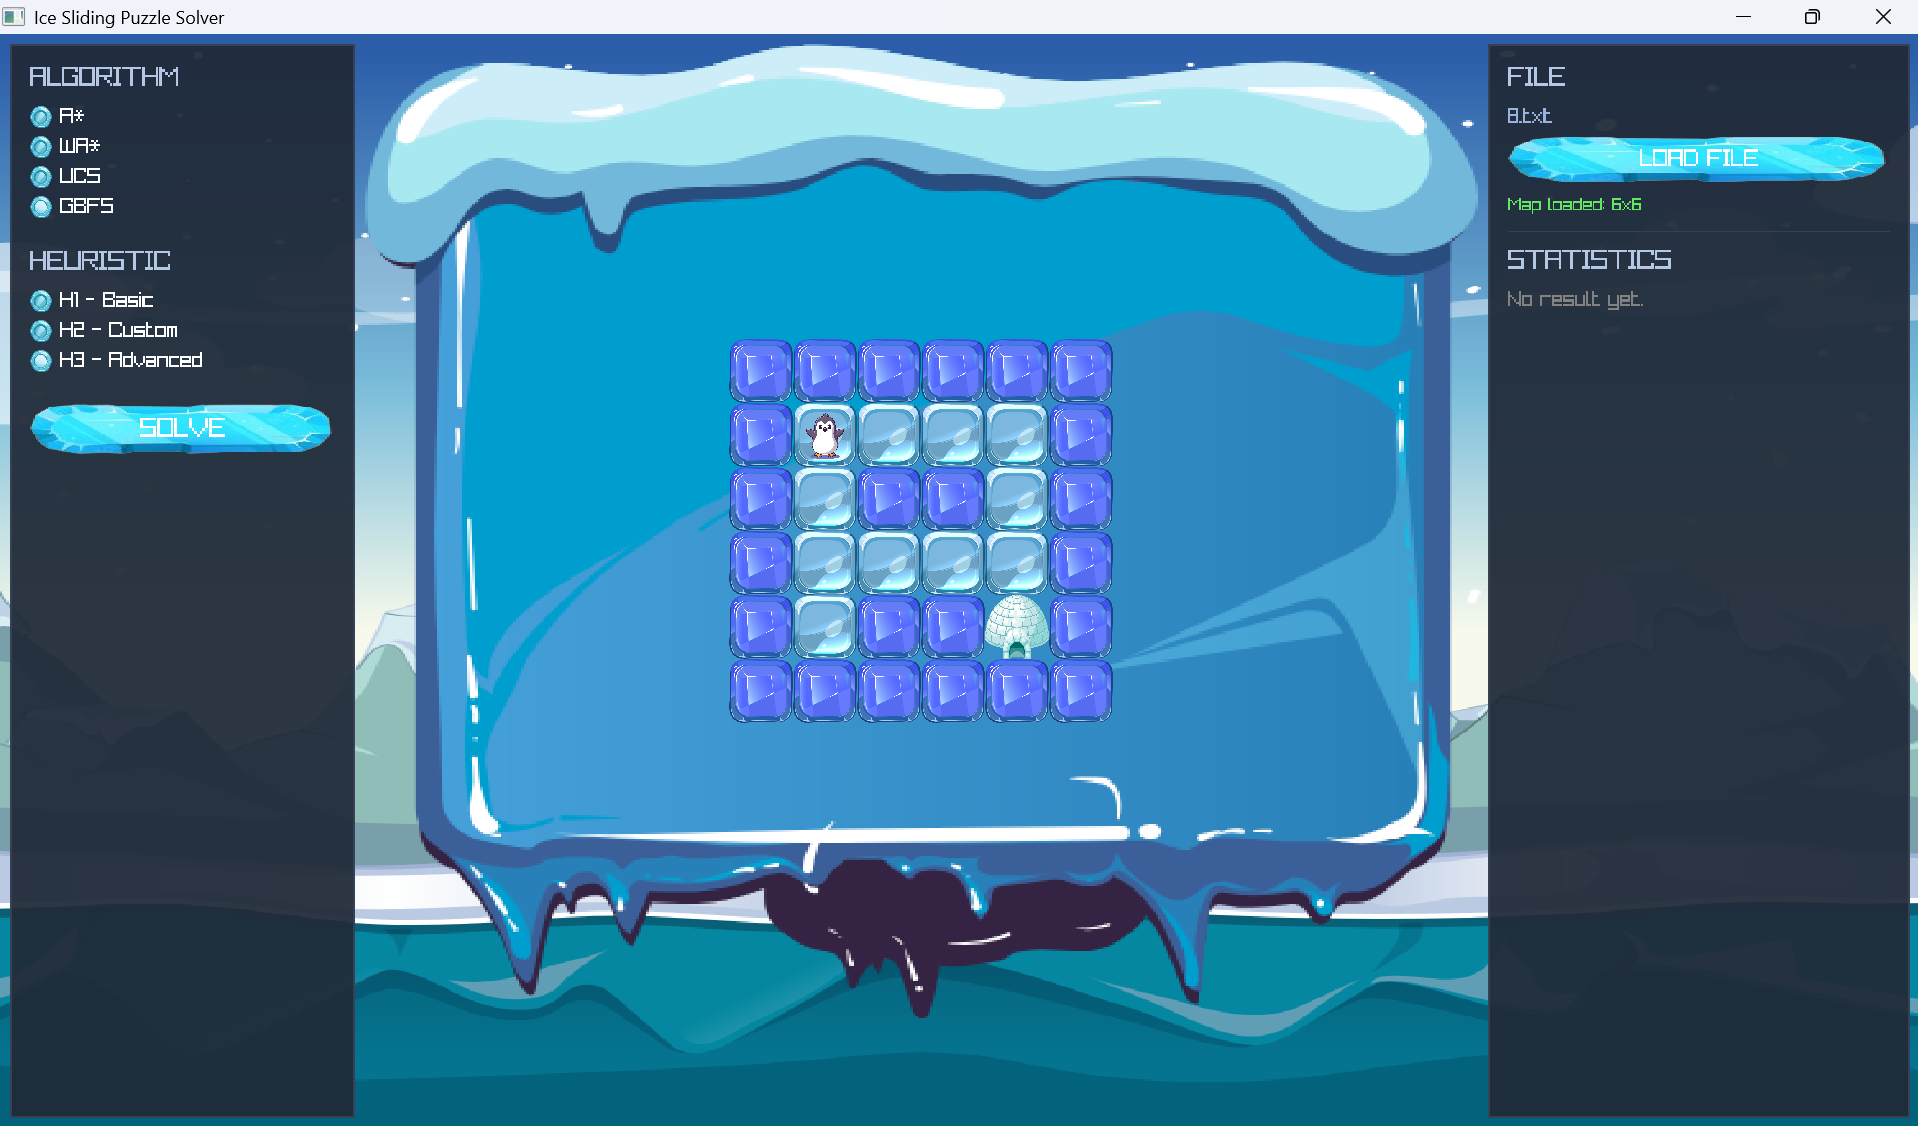
\includegraphics[width=0.55\textwidth]{public/map8.png}
	\caption{Visualisasi map pada Test Case 8}
\end{figure}

\begin{figure}[H]
	\centering
	\begin{minipage}{0.48\textwidth}
		\centering
		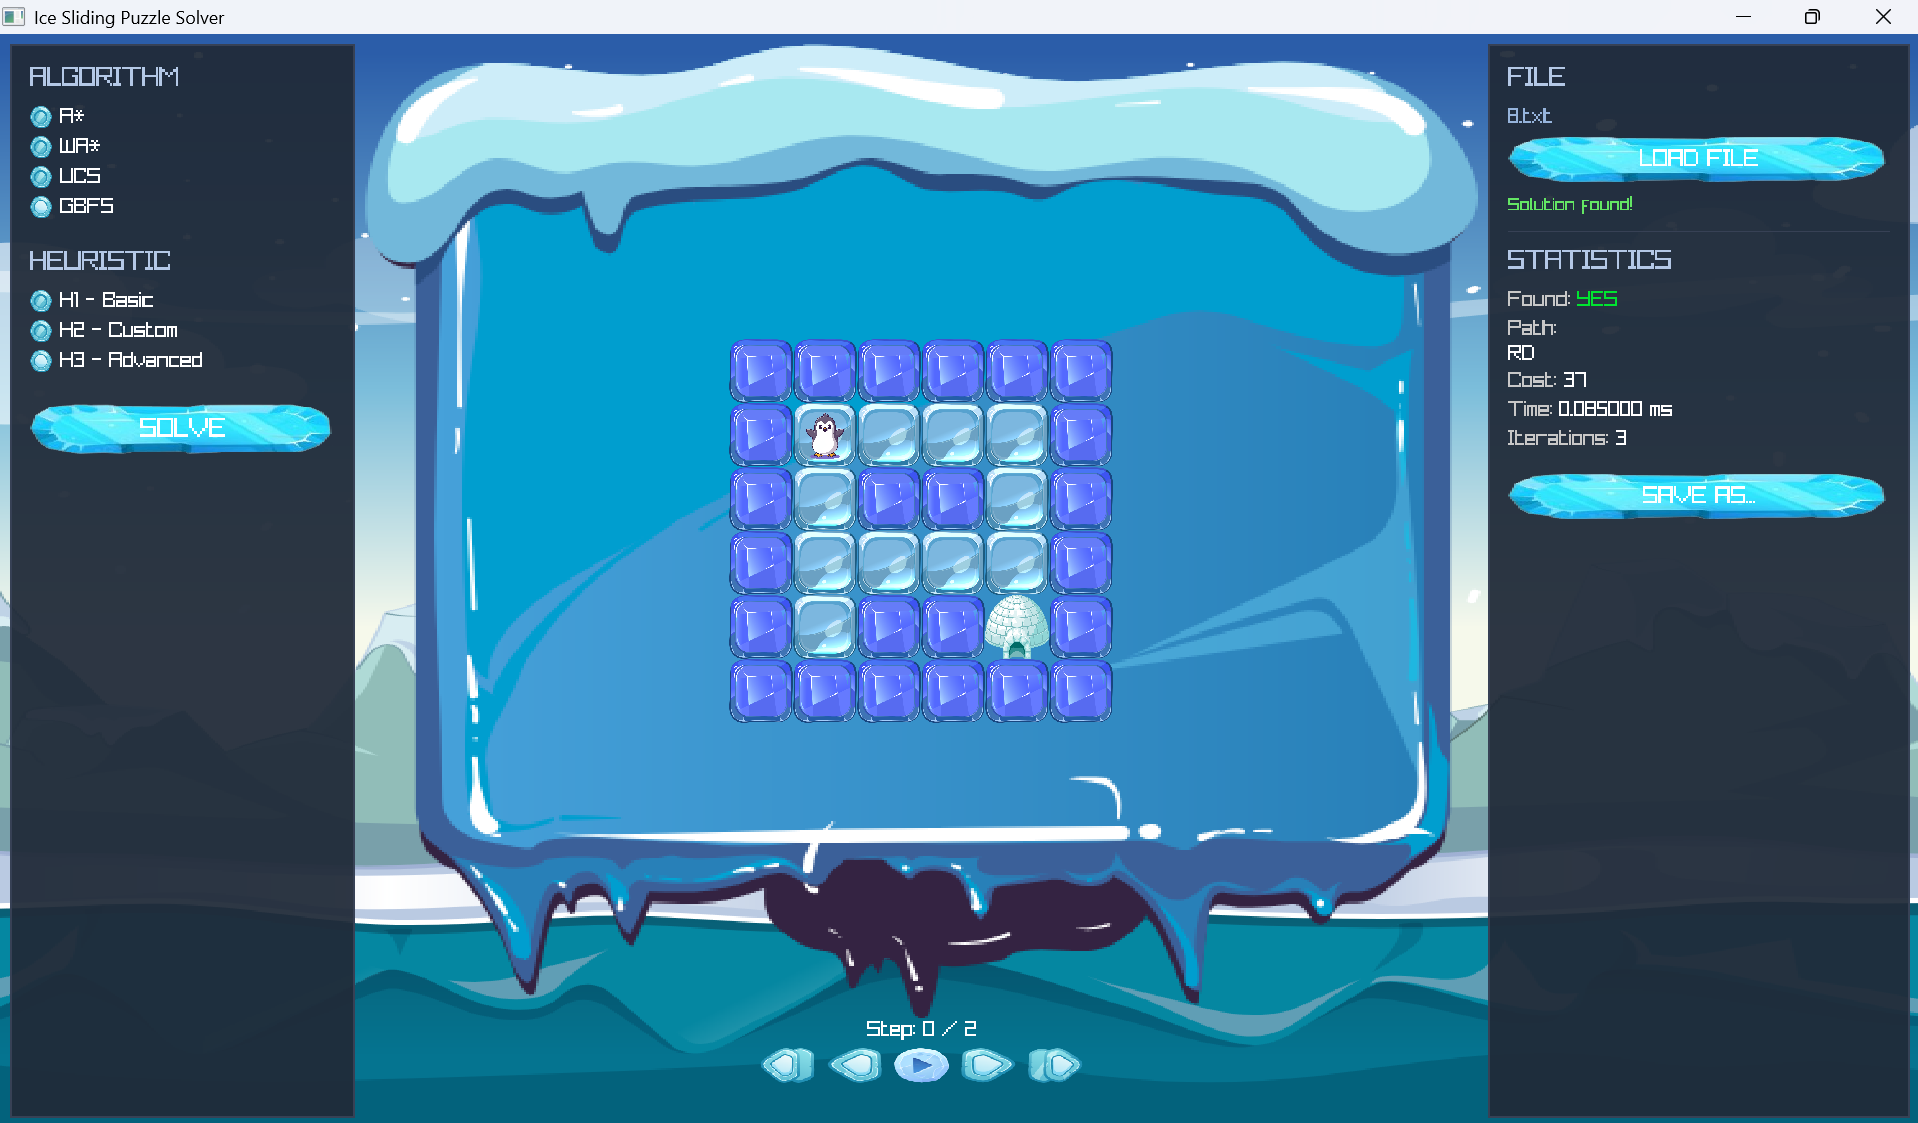
\includegraphics[width=\textwidth]{public/test8-GBFS-h3.png}
		\caption{Output Test 8 menggunakan GBFS + H3}
	\end{minipage}
	\hfill
	\begin{minipage}{0.48\textwidth}
		\centering
		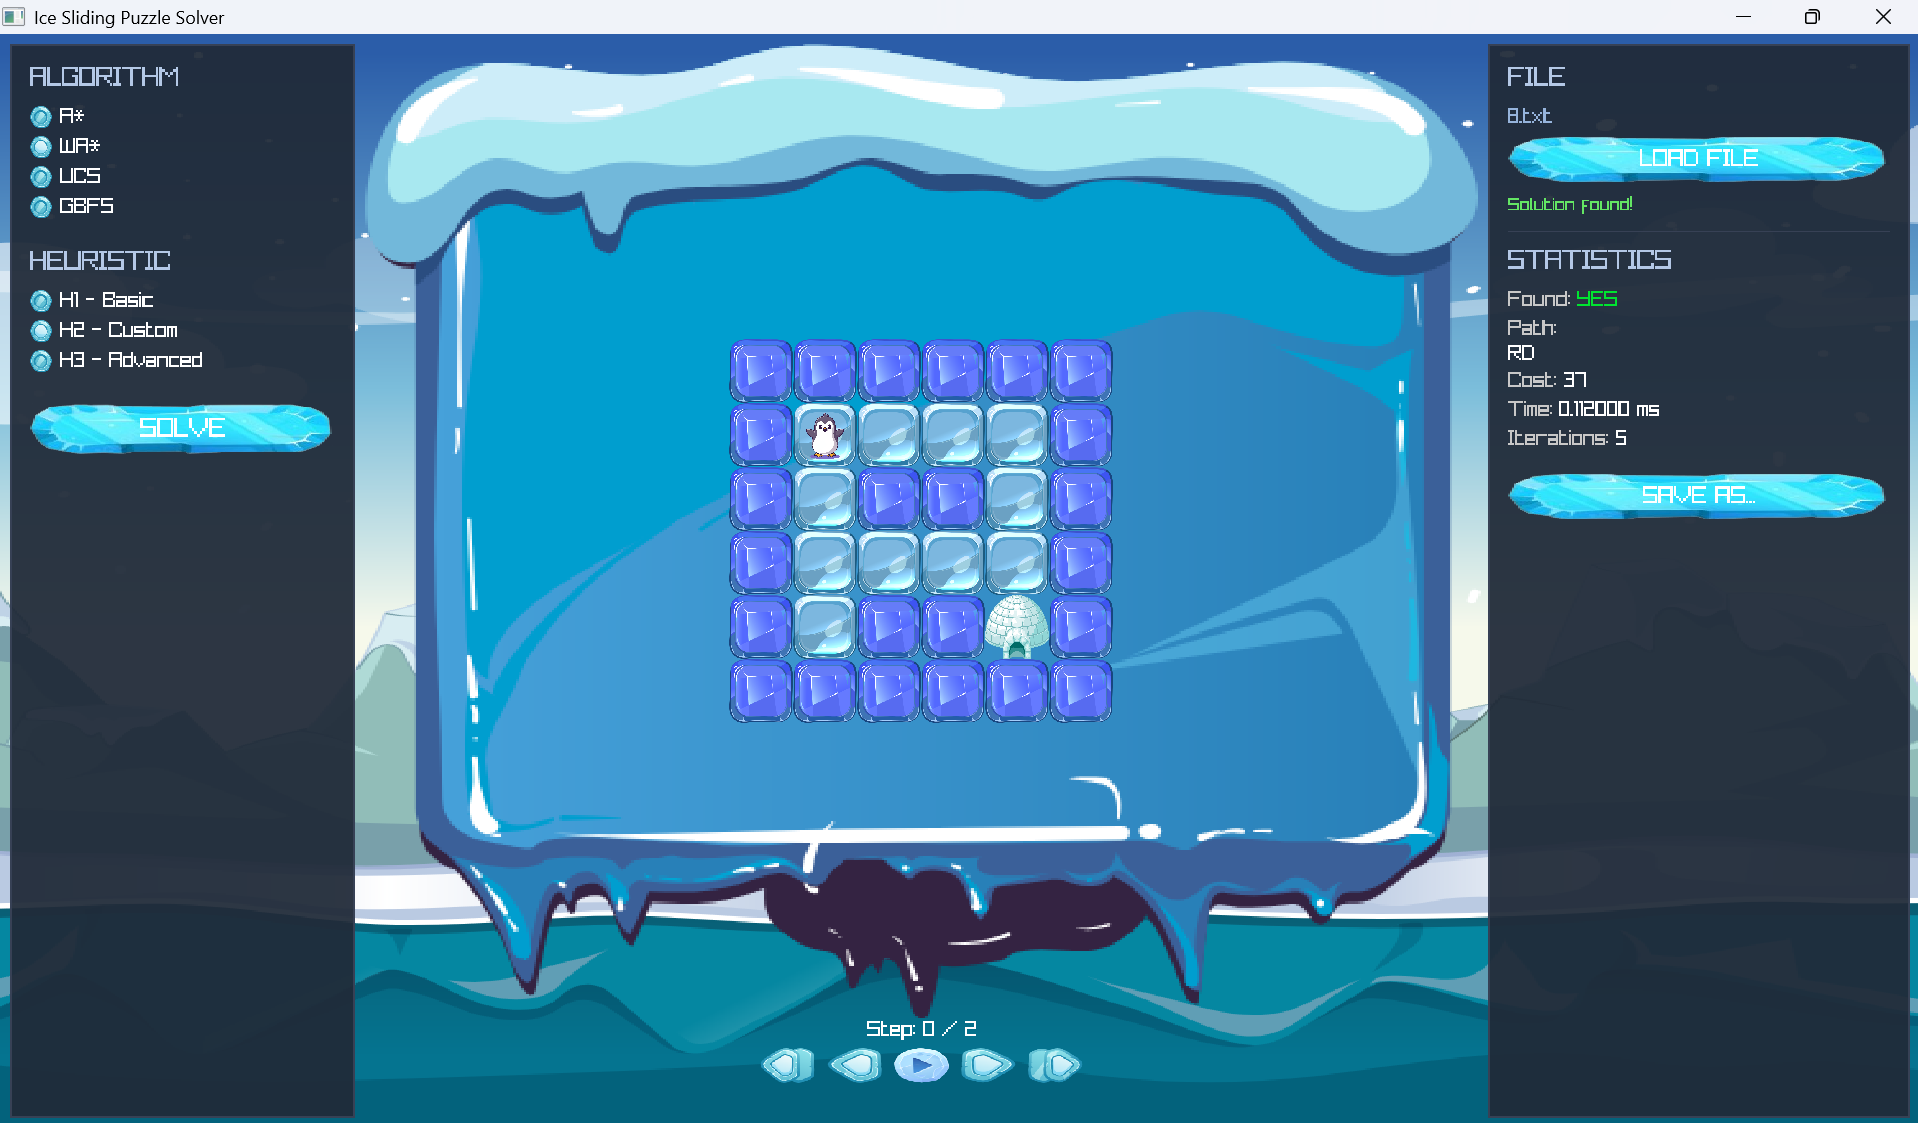
\includegraphics[width=\textwidth]{public/test8-WA-h2.png}
		\caption{Output Test 8 menggunakan Weighted A* + H2}
	\end{minipage}
\end{figure}

\begin{table}[H]
	\centering
	\caption{Hasil percobaan pada Test Case 8}
	\small
	\begin{tabular}{|p{4cm}|p{2.5cm}|p{2.5cm}|p{2.5cm}|}
		\hline
		\rowcolor{gray!20}
		\textbf{Algoritma} & \textbf{Cost} & \textbf{Time (ms)} & \textbf{Iterations} \\
		\hline
		A* - Basic & 37 & 0.124 & 5 \\
		\hline
		A* - Custom & 37 & 0.103 & 5 \\
		\hline
		A* - Advanced & 37 & 0.145 & 5 \\
		\hline
		WA* - Basic & 37 & 0.120 & 5 \\
		\hline
		WA* - Custom & 37 & 0.112 & 5 \\
		\hline
		WA* - Advanced & 37 & 0.120 & 5 \\
		\hline
		UCS & 37 & 0.102 & 4 \\
		\hline
		GBFS - Basic & 37 & 0.077 & 3 \\
		\hline
		GBFS - Custom & 37 & 0.093 & 3 \\
		\hline
		GBFS - Advanced & 37 & 0.085 & 3 \\
		\hline
	\end{tabular}
\end{table}

\begin{tcolorbox}[
	colback=green!5,
	colframe=green!50!black,
	title=\textbf{Ringkasan Test Case 8},
	arc=2mm,
	boxrule=0.8pt
]
Seluruh algoritma menghasilkan cost solusi yang sama, yaitu 37. 
Hal ini menunjukkan bahwa pada map sederhana tanpa angka dan lava, perbedaan algoritma lebih terlihat pada jumlah iterasi dan waktu eksekusi, bukan pada kualitas cost solusi.
\end{tcolorbox}


\subsection{Test Case 17}

\begin{tcolorbox}[
	colback=blue!5,
	colframe=blue!60!black,
	title=\textbf{Ringkasan Input Test Case 17},
	arc=2mm,
	boxrule=0.8pt
]
Test case 17 menggunakan papan berukuran $10 \times 10$ dengan banyak angka wajib dari \texttt{0} sampai \texttt{7}. 
Kasus ini digunakan untuk menguji kemampuan algoritma dalam mengikuti constraint angka berurutan sambil tetap memperhitungkan cost tile yang bervariasi.
\end{tcolorbox}

\begin{table}[H]
	\centering
	\caption{Karakteristik input Test Case 17}
	\begin{tabular}{|p{4cm}|p{9.5cm}|}
		\hline
		\rowcolor{blue!15}
		\textbf{Aspek} & \textbf{Keterangan} \\
		\hline
		Ukuran papan & $10 \times 10$ \\
		\hline
		Posisi awal & Ditandai dengan karakter \texttt{Z} pada bagian bawah map \\
		\hline
		Goal & Ditandai dengan karakter \texttt{O} \\
		\hline
		Angka wajib & Terdapat angka \texttt{0} sampai \texttt{7} yang harus dilalui berurutan \\
		\hline
		Lava & Tidak ada \\
		\hline
		Karakteristik utama & Map berisi banyak angka dan cost tile yang meningkat, sehingga cocok untuk menguji perbedaan cost solusi dan jumlah iterasi. \\
		\hline
	\end{tabular}
\end{table}

\begin{tcolorbox}[
	colback=gray!5,
	colframe=black!60,
	title=\textbf{Isi File \texttt{17.txt}},
	arc=2mm,
	boxrule=0.8pt
]
\tiny
\begin{verbatim}
10 10
XXXXXXXXXX
X***X****X
X*****3*XX
X********X
X***2**4*X
XX***5***X
X**1*X*X*X
X06******X
XZ***7*OXX
XXXXXXXXXX
999 999 999 999 999 999 999 999 999 999
999 5 2 3 999 6 7 8 9 999
999 1 10 11 12 13 14 15 999 999
999 17 18 19 20 21 22 23 24 999
999 25 26 27 28 29 30 31 32 999
999 999 34 35 36 37 38 39 40 999
999 41 42 43 44 999 46 999 48 999
999 49 50 51 52 53 54 55 56 999
999 57 58 59 60 61 62 63 999 999
999 999 999 999 999 999 999 999 999 999
\end{verbatim}
\end{tcolorbox}

\begin{figure}[H]
	\centering
	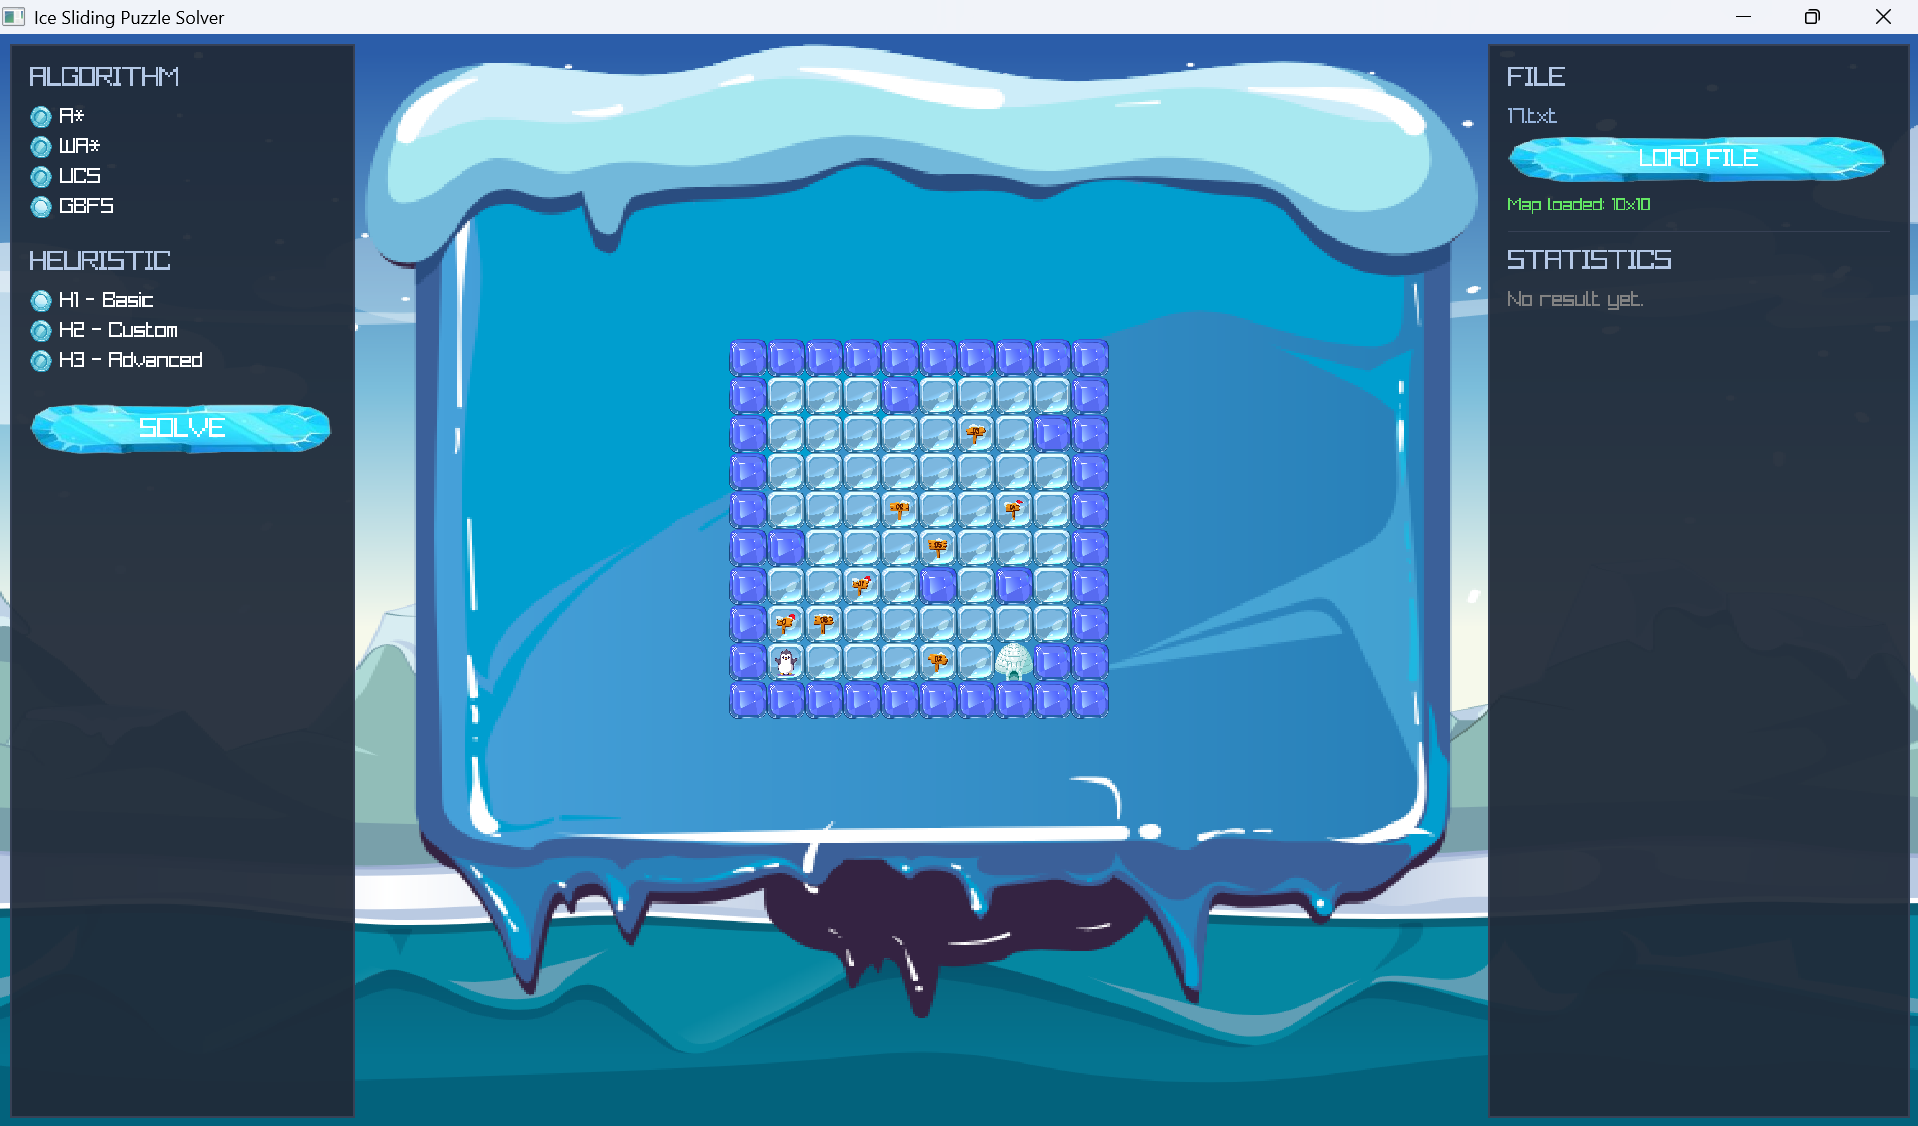
\includegraphics[width=0.65\textwidth]{public/map17.png}
	\caption{Visualisasi map pada Test Case 17}
\end{figure}

\begin{figure}[H]
	\centering
	\begin{minipage}{0.48\textwidth}
		\centering
		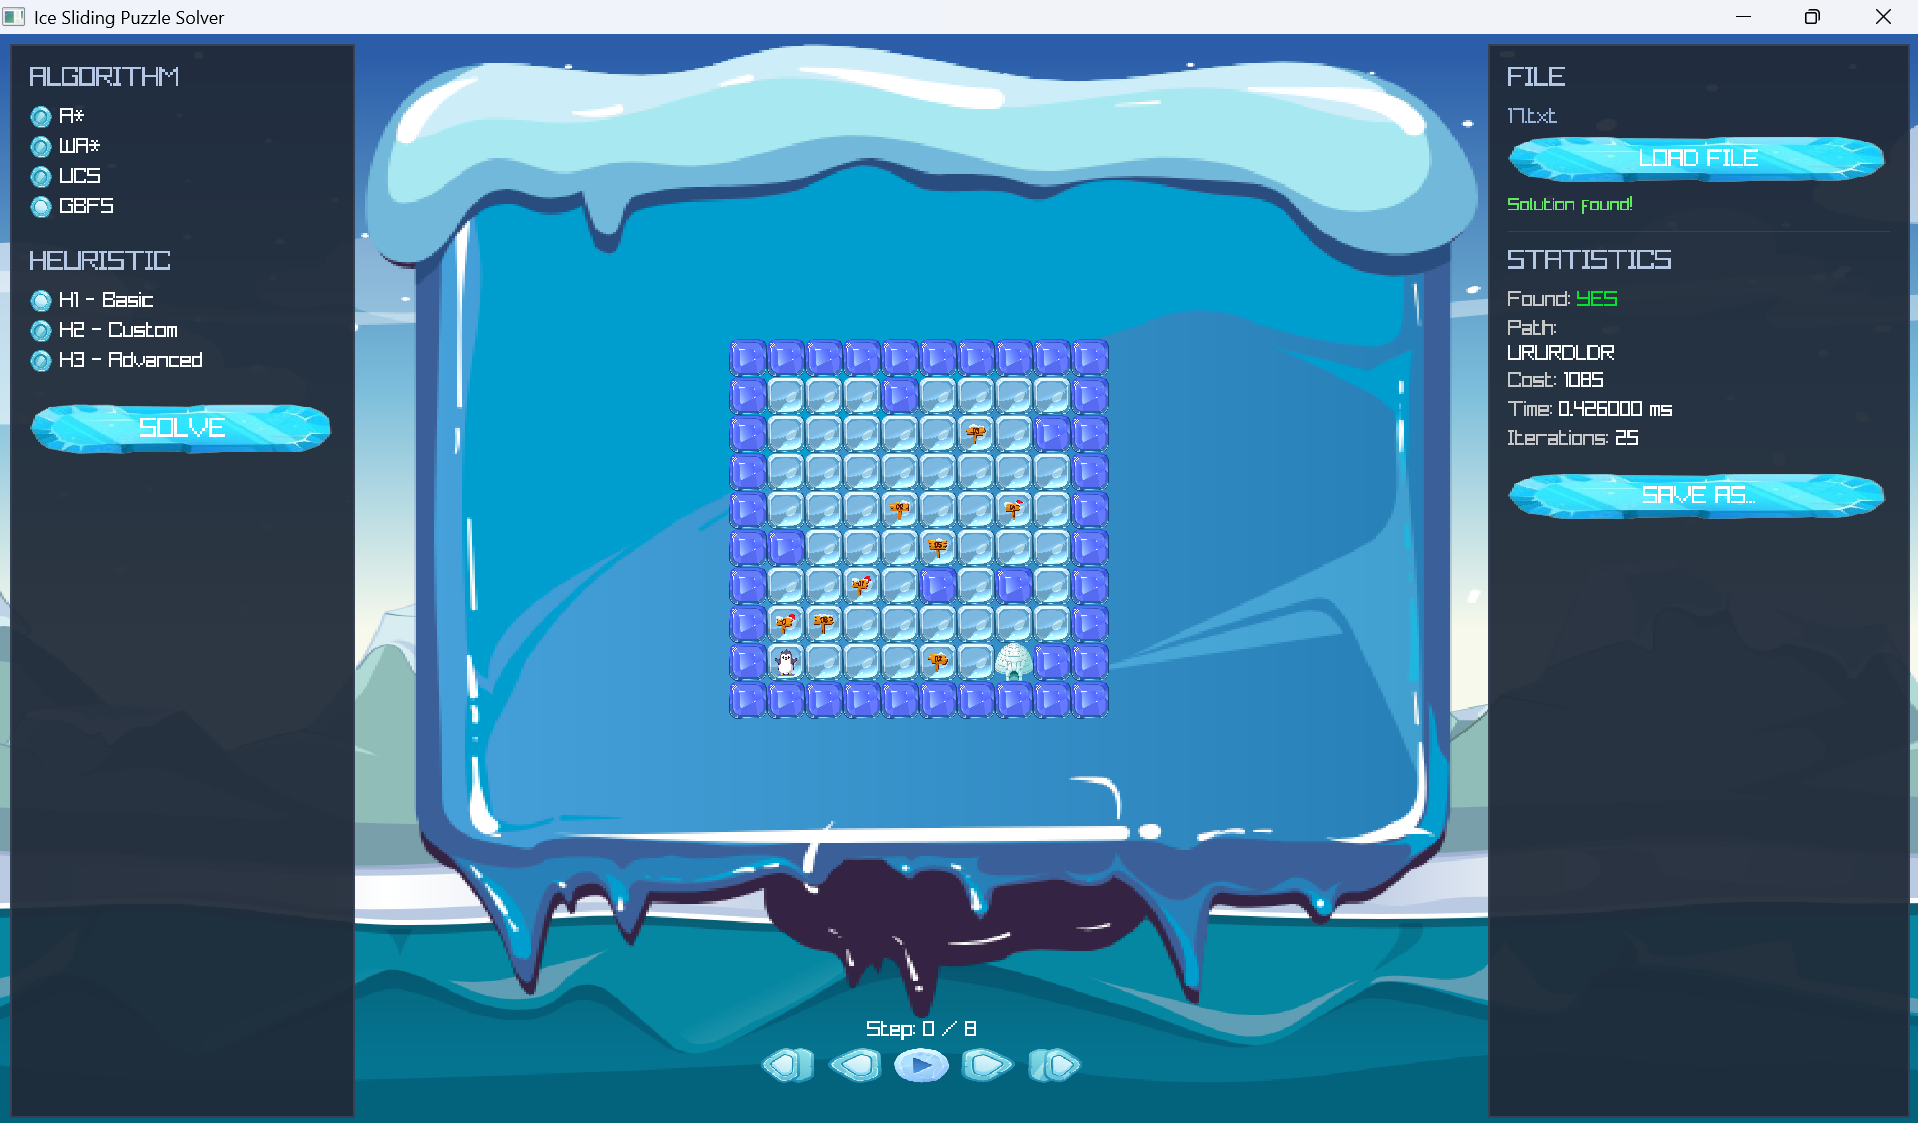
\includegraphics[width=\textwidth]{public/test17-GBFS-h1.png}
		\caption{Output Test 17 menggunakan GBFS + H1}
	\end{minipage}
	\hfill
	\begin{minipage}{0.48\textwidth}
		\centering
		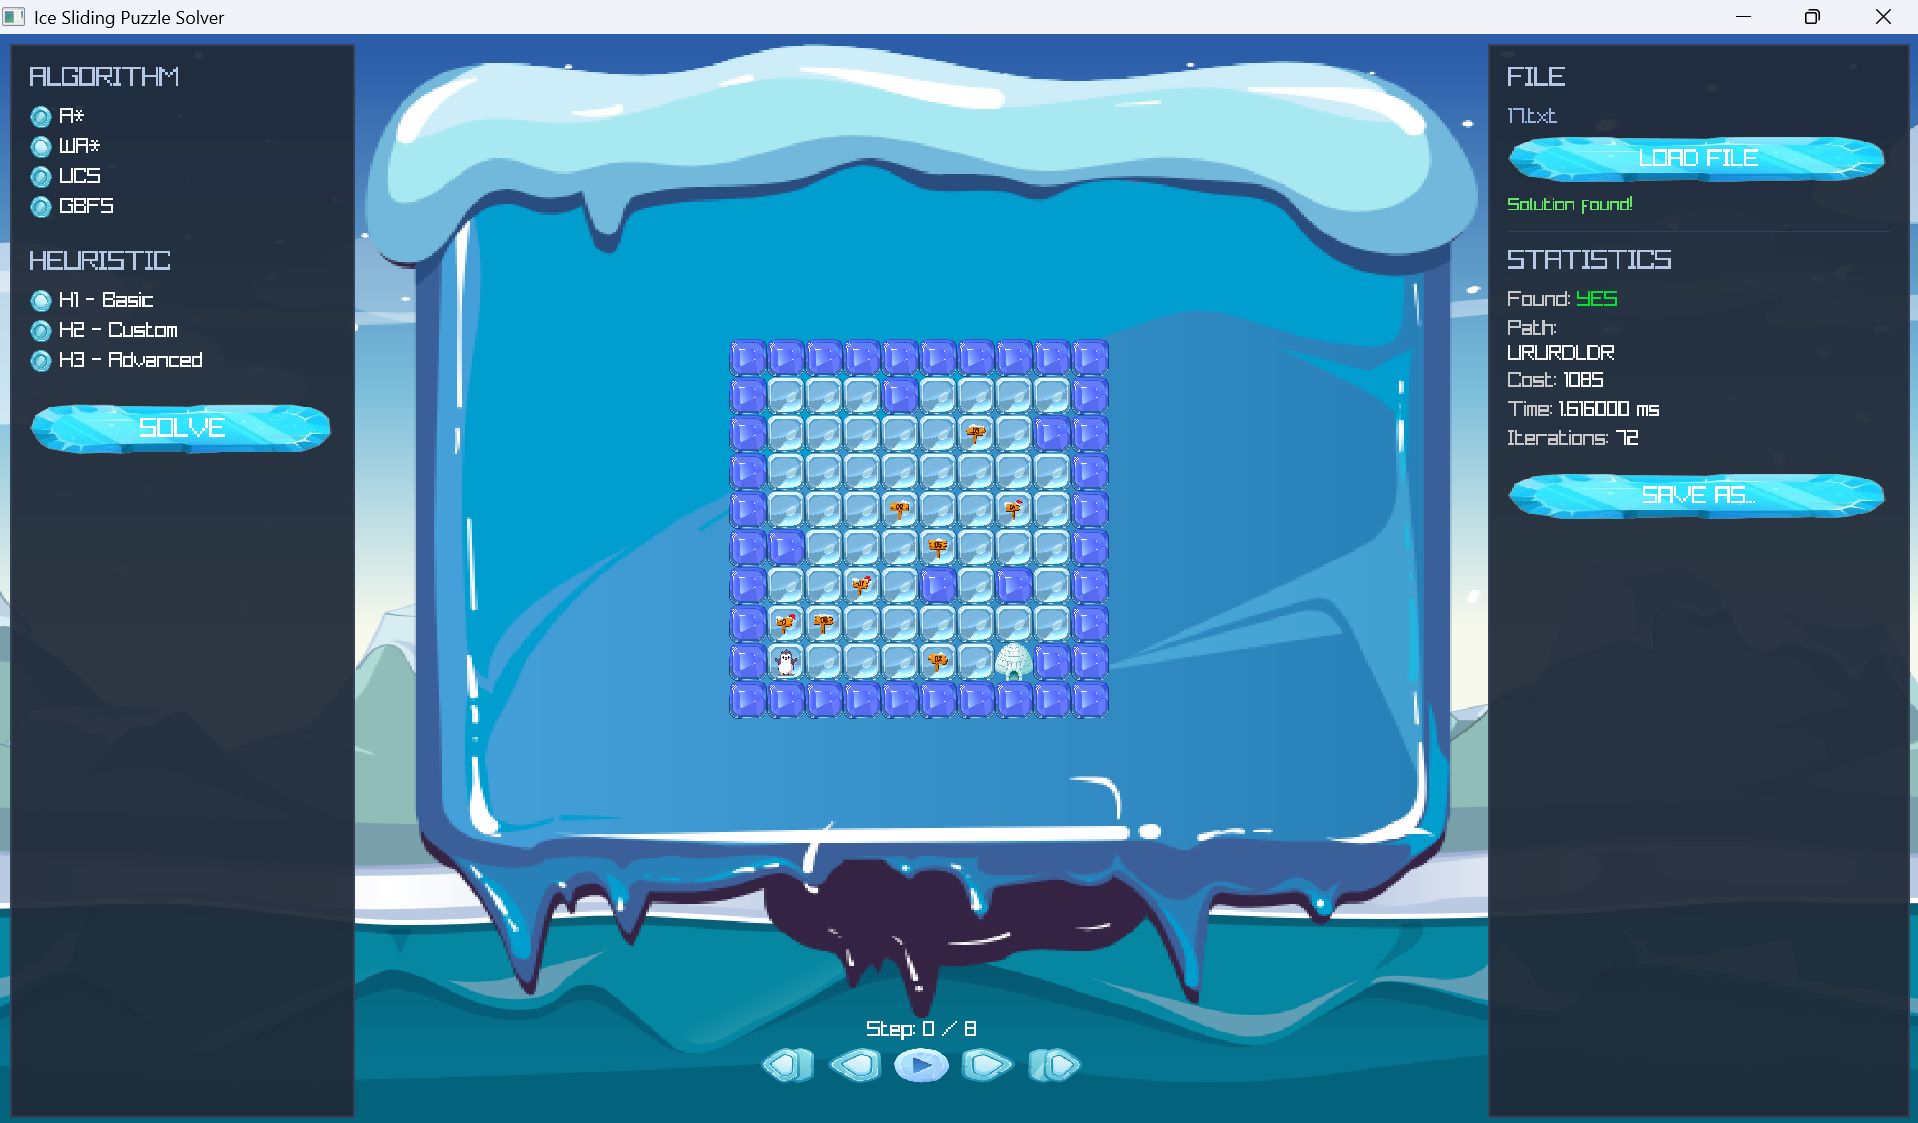
\includegraphics[width=\textwidth]{public/test17-WA-h1.png}
		\caption{Output Test 17 menggunakan Weighted A* + H1}
	\end{minipage}
\end{figure}

\begin{table}[H]
	\centering
	\caption{Hasil percobaan pada Test Case 17}
	\small
	\begin{tabular}{|p{4cm}|p{2.5cm}|p{2.5cm}|p{2.5cm}|}
		\hline
		\rowcolor{gray!20}
		\textbf{Algoritma} & \textbf{Cost} & \textbf{Time (ms)} & \textbf{Iterations} \\
		\hline
		A* - Basic & 1085 & 1.741 & 72 \\
		\hline
		A* - Custom & 1085 & 1.796 & 72 \\
		\hline
		A* - Advanced & 1085 & 2.639 & 72 \\
		\hline
		WA* - Basic & 1085 & 1.616 & 72 \\
		\hline
		WA* - Custom & 1085 & 2.232 & 72 \\
		\hline
		WA* - Advanced & 1085 & 2.581 & 72 \\
		\hline
		UCS & 1085 & 1.228 & 71 \\
		\hline
		GBFS - Basic & 1085 & 0.552 & 25 \\
		\hline
		GBFS - Custom & 1085 & 0.439 & 11 \\
		\hline
		GBFS - Advanced & 1085 & 0.534 & 10 \\
		\hline
	\end{tabular}
\end{table}

\begin{tcolorbox}[
	colback=green!5,
	colframe=green!50!black,
	title=\textbf{Ringkasan Test Case 17},
	arc=2mm,
	boxrule=0.8pt
]
Semua algoritma menghasilkan cost solusi yang sama, yaitu 1085. 
Namun, GBFS dengan heuristik Custom dan Advanced meninjau jumlah iterasi yang jauh lebih sedikit dibanding UCS, A*, dan Weighted A*. 
Hal ini menunjukkan bahwa pada map ini, heuristik mampu mengarahkan pencarian secara efektif.
\end{tcolorbox}


\subsection{Test Case 20}

\begin{tcolorbox}[
	colback=blue!5,
	colframe=blue!60!black,
	title=\textbf{Ringkasan Input Test Case 20},
	arc=2mm,
	boxrule=0.8pt
]
Test case 20 menggunakan papan berukuran $12 \times 12$ dengan pola obstacle yang menyerupai labirin. 
Tidak terdapat angka wajib maupun lava, sehingga pengujian difokuskan pada kemampuan algoritma mencari lintasan sliding yang valid di antara banyak rintangan.
\end{tcolorbox}

\begin{table}[H]
	\centering
	\caption{Karakteristik input Test Case 20}
	\begin{tabular}{|p{4cm}|p{9.5cm}|}
		\hline
		\rowcolor{blue!15}
		\textbf{Aspek} & \textbf{Keterangan} \\
		\hline
		Ukuran papan & $12 \times 12$ \\
		\hline
		Posisi awal & Ditandai dengan karakter \texttt{Z} pada kiri atas area bebas \\
		\hline
		Goal & Ditandai dengan karakter \texttt{O} pada kanan bawah area bebas \\
		\hline
		Angka wajib & Tidak ada \\
		\hline
		Lava & Tidak ada \\
		\hline
		Karakteristik utama & Map labirin dengan banyak obstacle, sehingga menguji kemampuan algoritma menemukan jalur sliding yang tidak langsung. \\
		\hline
	\end{tabular}
\end{table}

\begin{tcolorbox}[
	colback=gray!5,
	colframe=black!60,
	title=\textbf{Isi File \texttt{20.txt}},
	arc=2mm,
	boxrule=0.8pt
]
\tiny
\begin{verbatim}
12 12
XXXXXXXXXXXX
XZ*********X
X*XXXXXXXX*X
X*X******X*X
X*X*XXXX*X*X
X*X*X**X*X*X
X*X*X**X*X*X
X*X*XXXX*X*X
X*X******X*X
X*XXXXXXXX*X
X*********OX
XXXXXXXXXXXX
999 999 999 999 999 999 999 999 999 999 999 999
999 1 2 3 4 5 6 7 8 9 10 999
999 11 999 999 999 999 999 999 999 999 12 999
999 13 999 14 15 16 17 18 19 20 999 999
999 21 999 22 999 999 23 24 999 25 999 999
999 26 999 27 999 28 29 999 30 31 999 999
999 32 999 33 999 34 35 999 36 37 999 999
999 38 999 39 999 999 40 41 999 42 999 999
999 43 999 44 45 46 47 48 49 50 999 999
999 51 999 999 999 999 999 999 999 999 52 999
999 53 54 55 56 57 58 59 60 61 62 999
999 999 999 999 999 999 999 999 999 999 999 999
\end{verbatim}
\end{tcolorbox}

\begin{figure}[H]
	\centering
	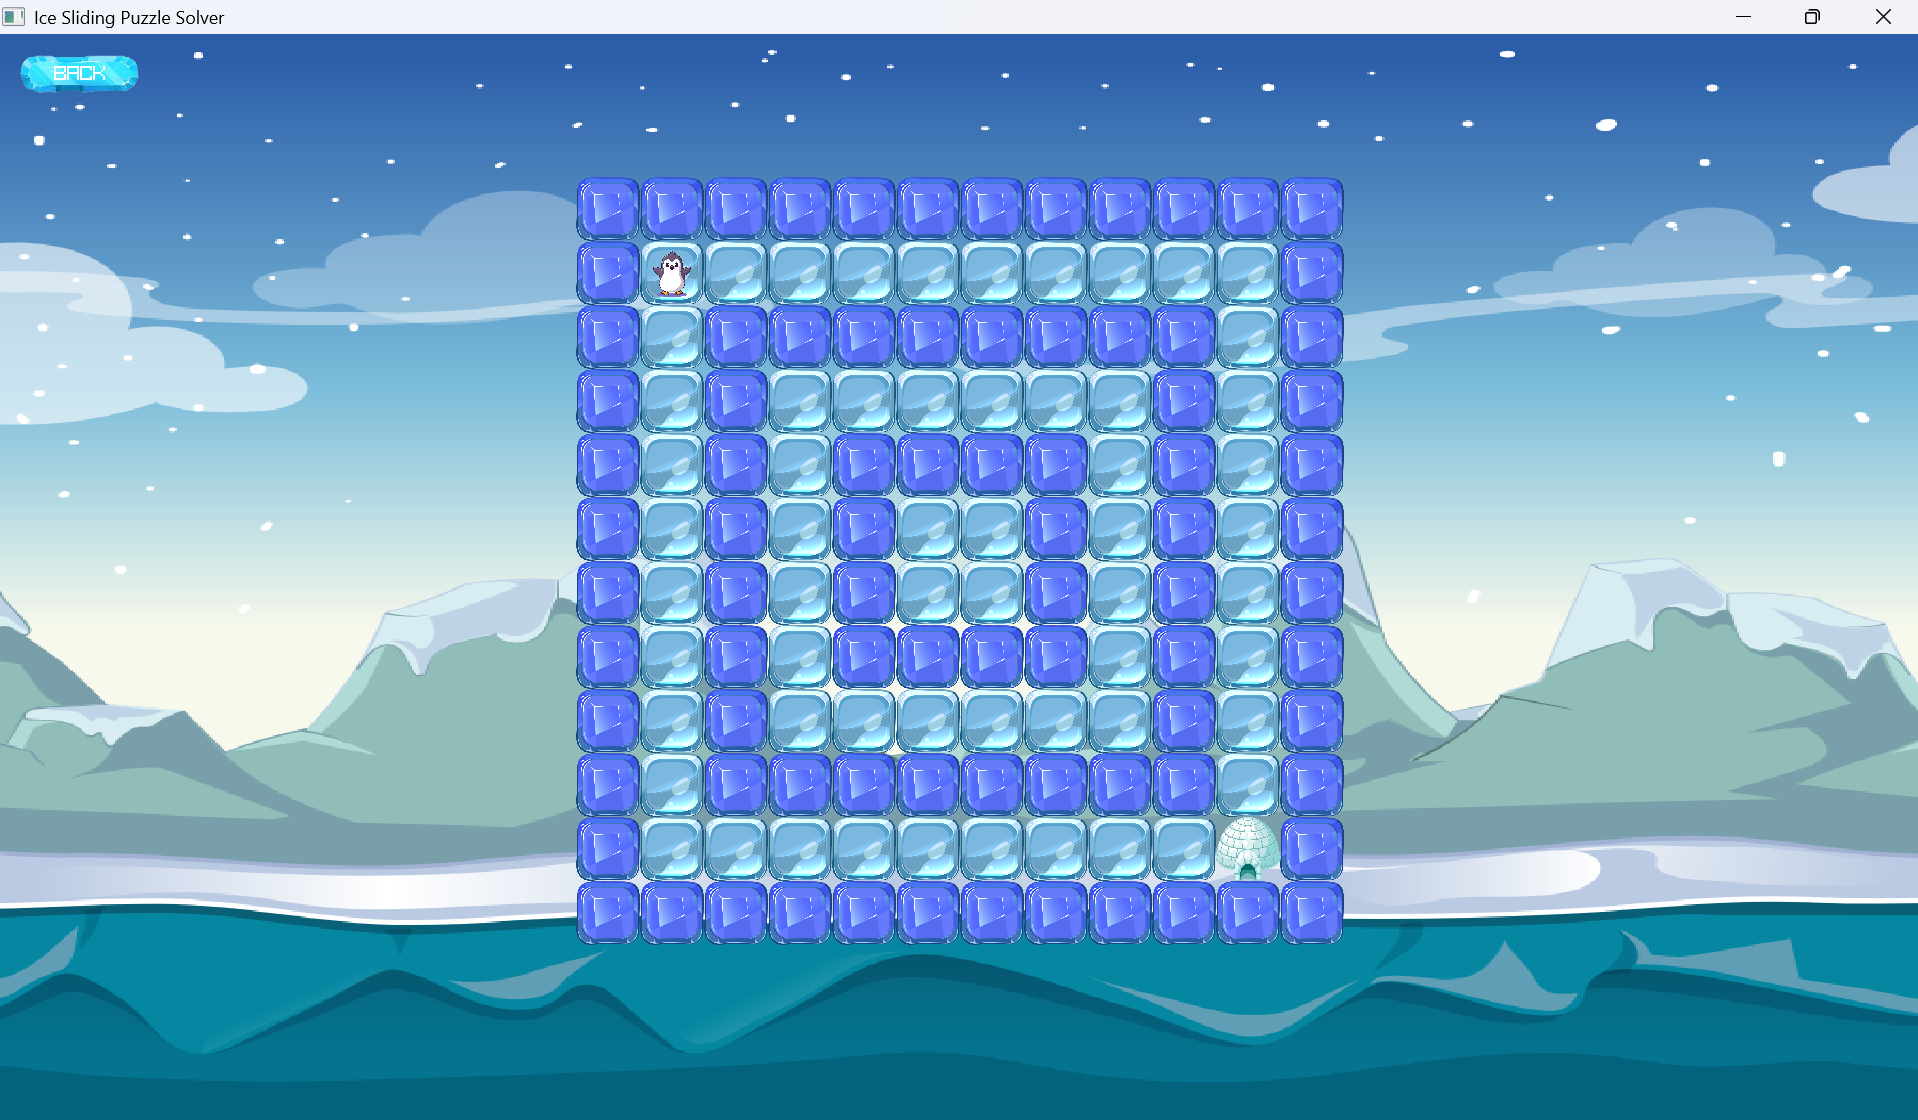
\includegraphics[width=0.65\textwidth]{public/map-20.png}
	\caption{Visualisasi map pada Test Case 20}
\end{figure}

\begin{figure}[H]
	\centering
	\begin{minipage}{0.48\textwidth}
		\centering
		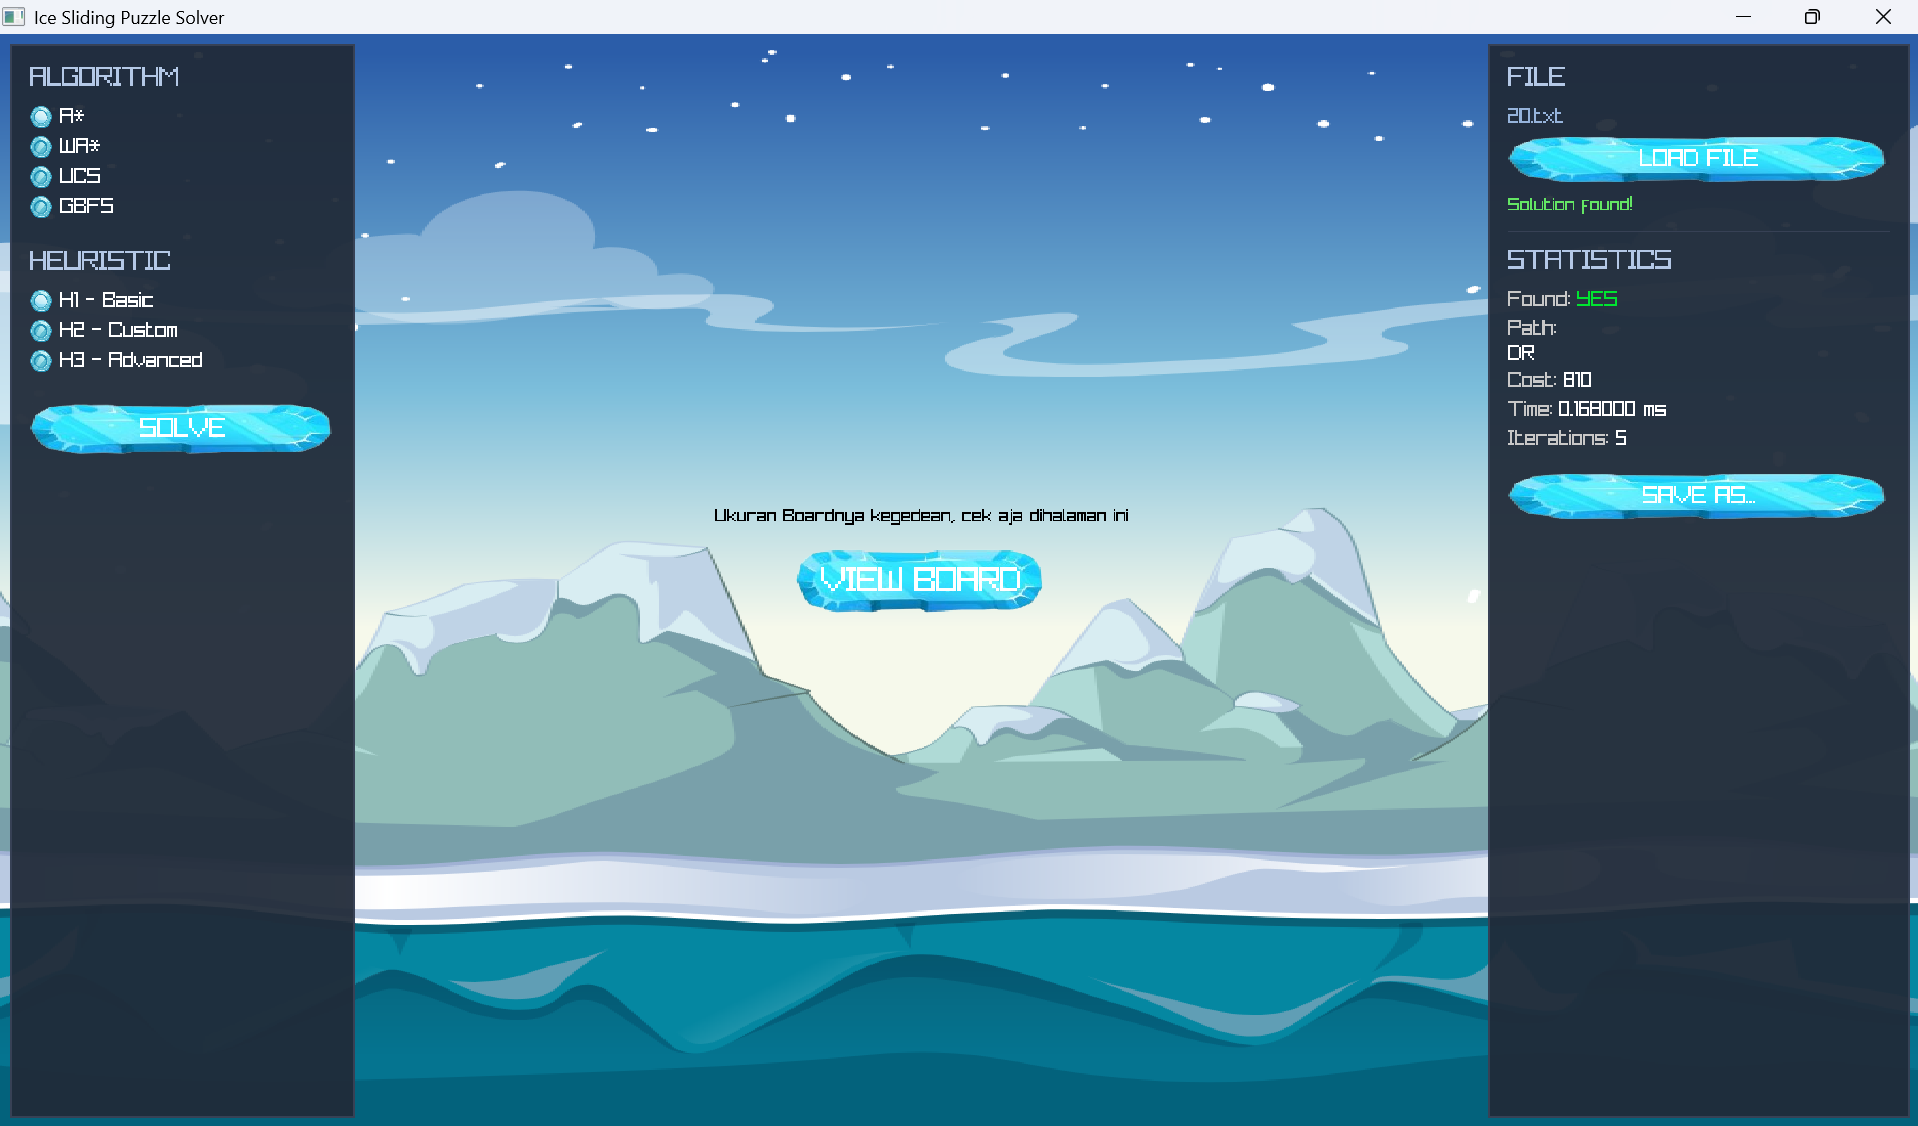
\includegraphics[width=\textwidth]{public/test20-A-h1.png}
		\caption{Output Test 20 menggunakan A* + H1}
	\end{minipage}
	\hfill
	\begin{minipage}{0.48\textwidth}
		\centering
		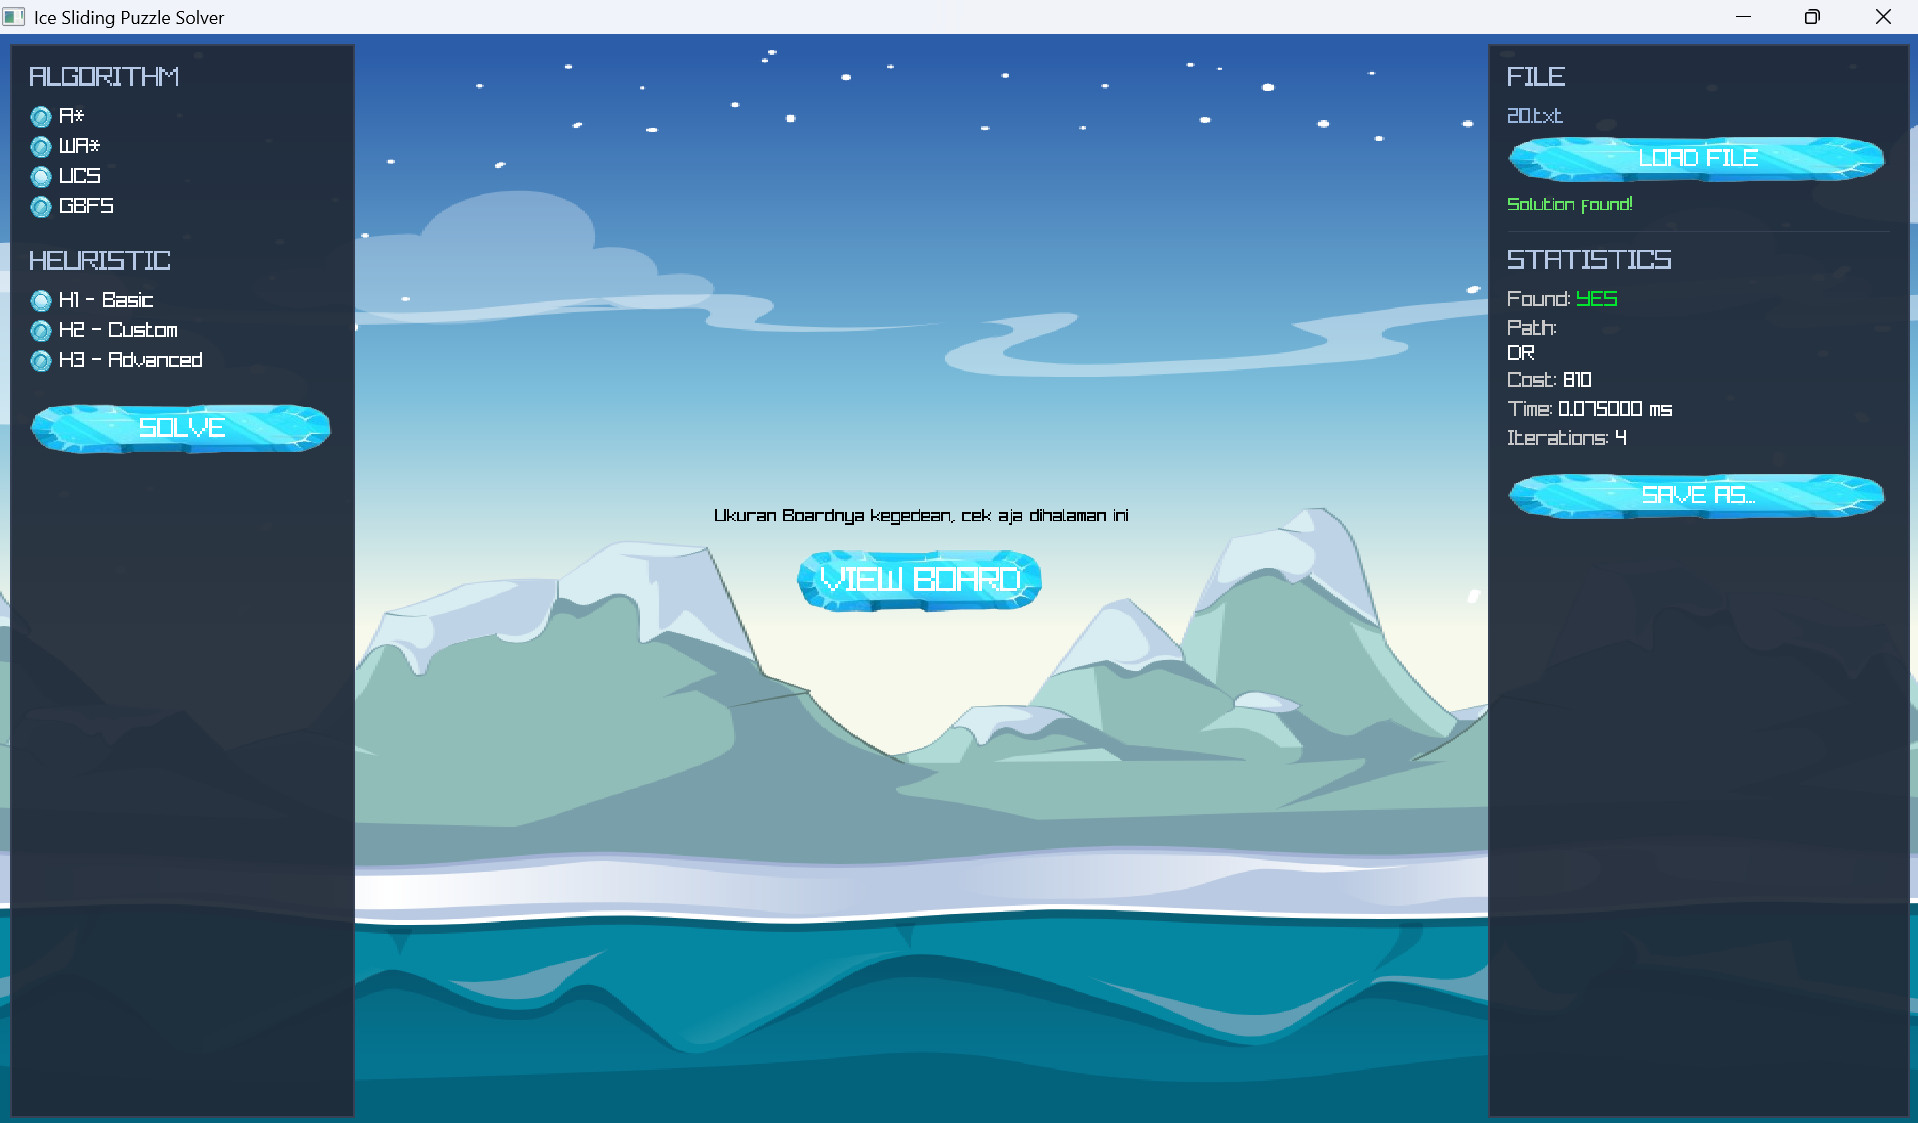
\includegraphics[width=\textwidth]{public/test20-UCS.png}
		\caption{Output Test 20 menggunakan UCS}
	\end{minipage}
\end{figure}

\begin{table}[H]
	\centering
	\caption{Hasil percobaan pada Test Case 20}
	\small
	\begin{tabular}{|p{4cm}|p{2.5cm}|p{2.5cm}|p{2.5cm}|}
		\hline
		\rowcolor{gray!20}
		\textbf{Algoritma} & \textbf{Cost} & \textbf{Time (ms)} & \textbf{Iterations} \\
		\hline
		A* - Basic & 810 & 0.196 & 5 \\
		\hline
		A* - Custom & 810 & 0.250 & 5 \\
		\hline
		A* - Advanced & 810 & 0.203 & 5 \\
		\hline
		WA* - Basic & 810 & 0.110 & 5 \\
		\hline
		WA* - Custom & 810 & 0.380 & 5 \\
		\hline
		WA* - Advanced & 810 & 0.246 & 5 \\
		\hline
		UCS & 810 & 0.113 & 4 \\
		\hline
		GBFS - Basic & 6174 & 0.065 & 3 \\
		\hline
		GBFS - Custom & 6174 & 0.136 & 3 \\
		\hline
		GBFS - Advanced & 6174 & 0.132 & 3 \\
		\hline
	\end{tabular}
\end{table}

\begin{tcolorbox}[
	colback=orange!5,
	colframe=orange!70!black,
	title=\textbf{Ringkasan Test Case 20},
	arc=2mm,
	boxrule=0.8pt
]
Pada test case ini, UCS, A*, dan Weighted A* menghasilkan cost 810, sedangkan GBFS menghasilkan cost 6174. 
Hal ini menunjukkan bahwa GBFS dapat menemukan solusi lebih cepat dari sisi iterasi, tetapi tidak selalu menghasilkan cost minimum karena hanya mengikuti estimasi heuristik.
\end{tcolorbox}


\subsection{Test Case 24}

\begin{tcolorbox}[
	colback=blue!5,
	colframe=blue!60!black,
	title=\textbf{Ringkasan Input Test Case 24},
	arc=2mm,
	boxrule=0.8pt
]
Test case 24 menggunakan papan berukuran $7 \times 12$ yang memiliki angka wajib dan beberapa lava. 
Kasus ini menguji dua aturan penting sekaligus, yaitu angka harus dilewati secara berurutan dan jalur yang melewati lava harus dianggap tidak valid.
\end{tcolorbox}

\begin{table}[H]
	\centering
	\caption{Karakteristik input Test Case 24}
	\begin{tabular}{|p{4cm}|p{9.5cm}|}
		\hline
		\rowcolor{blue!15}
		\textbf{Aspek} & \textbf{Keterangan} \\
		\hline
		Ukuran papan & $7 \times 12$ \\
		\hline
		Posisi awal & Ditandai dengan karakter \texttt{Z} pada sisi kiri map \\
		\hline
		Goal & Ditandai dengan karakter \texttt{O} pada sisi kanan bawah map \\
		\hline
		Angka wajib & Terdapat angka \texttt{0} sampai \texttt{6} yang harus dilalui berurutan \\
		\hline
		Lava & Ada beberapa tile \texttt{L} yang menyebabkan game over jika dilewati \\
		\hline
		Karakteristik utama & Kombinasi angka, obstacle, dan lava sehingga cocok untuk menguji validasi path dan constraint urutan angka. \\
		\hline
	\end{tabular}
\end{table}

\begin{tcolorbox}[
	colback=gray!5,
	colframe=black!60,
	title=\textbf{Isi File \texttt{24.txt}},
	arc=2mm,
	boxrule=0.8pt
]
\tiny
\begin{verbatim}
7 12
XXXXXXXXXXXX
XZ01*******X
X**L**X*L**X
X****4**3*2X
X5*X***L**XX
X***6*****OX
XXXXXXXXXXXX
999 999 999 999 999 999 999 999 999 999 999 999
999 1 2 3 4 5 6 7 8 9 10 999
999 11 12 999 13 14 999 15 999 16 17 999
999 18 19 20 21 22 23 24 25 26 27 999
999 28 29 999 30 31 32 999 33 34 999 999
999 35 36 37 38 39 40 41 42 43 44 999
999 999 999 999 999 999 999 999 999 999 999 999
\end{verbatim}
\end{tcolorbox}

\begin{figure}[H]
	\centering
	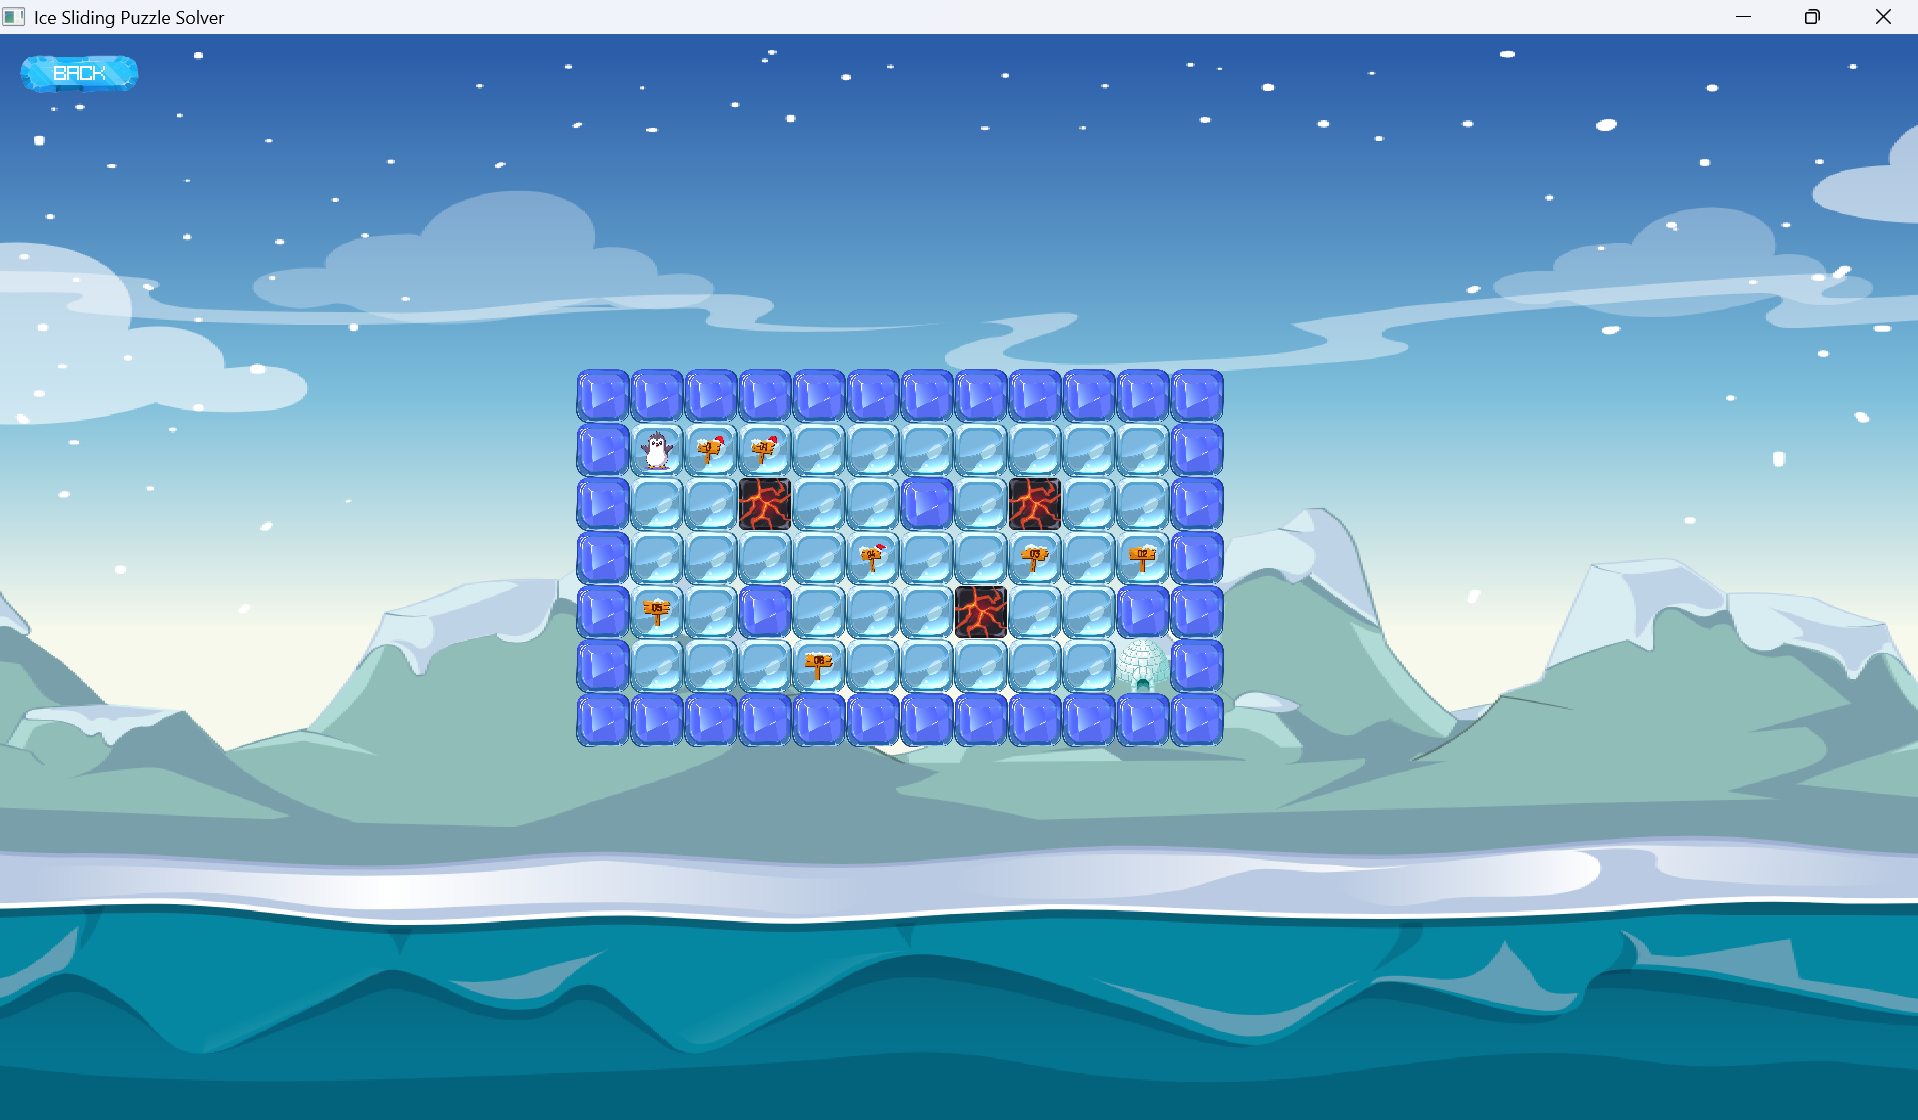
\includegraphics[width=0.75\textwidth]{public/map24.png}
	\caption{Visualisasi map pada Test Case 24}
\end{figure}

\begin{figure}[H]
	\centering
	\begin{minipage}{0.48\textwidth}
		\centering
		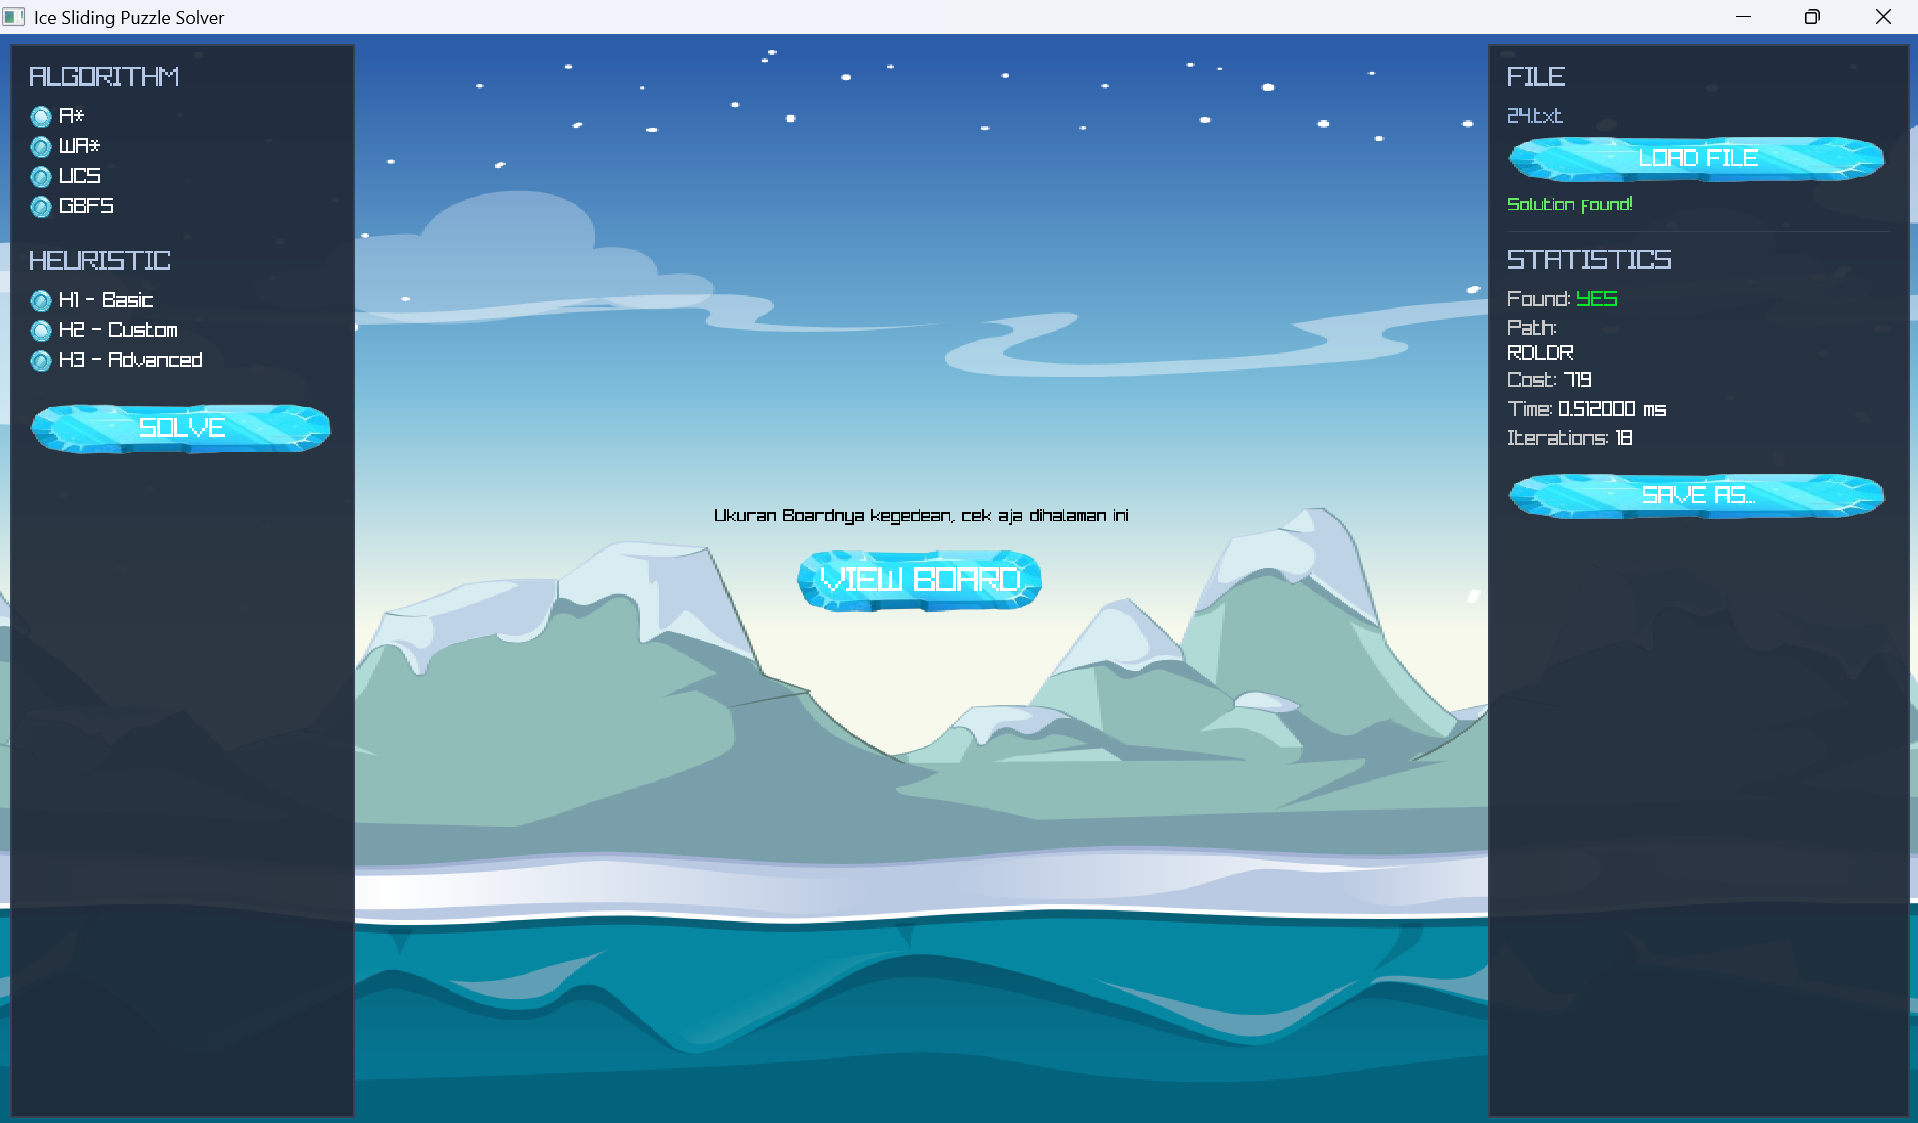
\includegraphics[width=\textwidth]{public/test24-A-h2.png}
		\caption{Output Test 24 menggunakan A* + H2}
	\end{minipage}
	\hfill
	\begin{minipage}{0.48\textwidth}
		\centering
		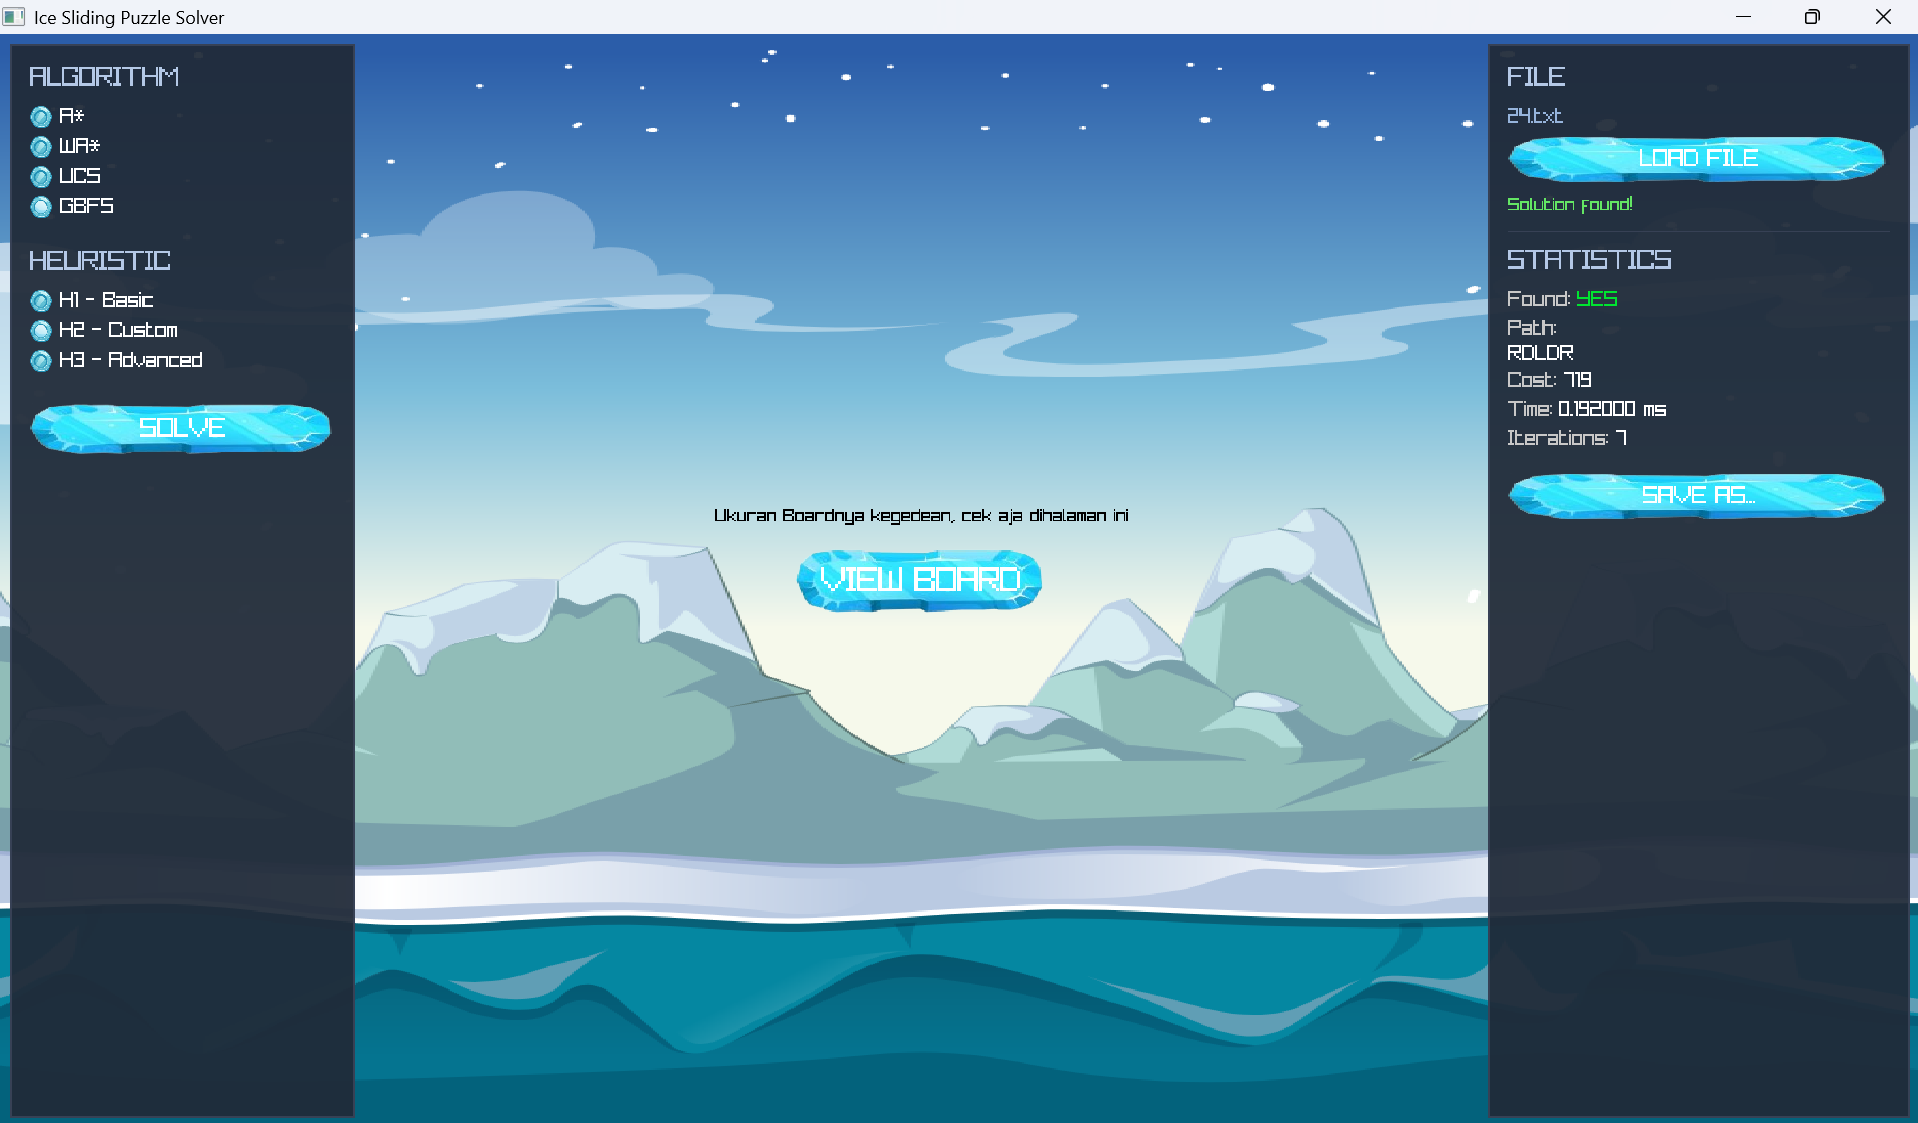
\includegraphics[width=\textwidth]{public/test24-GBFS-h2.png}
		\caption{Output Test 24 menggunakan GBFS + H2}
	\end{minipage}
\end{figure}

\begin{table}[H]
	\centering
	\caption{Hasil percobaan pada Test Case 24}
	\small
	\begin{tabular}{|p{4cm}|p{2.5cm}|p{2.5cm}|p{2.5cm}|}
		\hline
		\rowcolor{gray!20}
		\textbf{Algoritma} & \textbf{Cost} & \textbf{Time (ms)} & \textbf{Iterations} \\
		\hline
		A* - Basic & 719 & 0.229 & 17 \\
		\hline
		A* - Custom & 719 & 0.619 & 18 \\
		\hline
		A* - Advanced & 719 & 0.672 & 17 \\
		\hline
		WA* - Basic & 719 & 0.405 & 17 \\
		\hline
		WA* - Custom & 719 & 0.621 & 17 \\
		\hline
		WA* - Advanced & 719 & 0.534 & 17 \\
		\hline
		UCS & 719 & 0.339 & 17 \\
		\hline
		GBFS - Basic & 719 & 0.208 & 9 \\
		\hline
		GBFS - Custom & 719 & 0.192 & 7 \\
		\hline
		GBFS - Advanced & 719 & 0.356 & 7 \\
		\hline
	\end{tabular}
\end{table}

\begin{tcolorbox}[
	colback=green!5,
	colframe=green!50!black,
	title=\textbf{Ringkasan Test Case 24},
	arc=2mm,
	boxrule=0.8pt
]
Seluruh algoritma menghasilkan cost solusi yang sama, yaitu 719. 
GBFS dengan heuristik Custom dan Advanced memiliki jumlah iterasi paling kecil, yaitu 7 iterasi. 
Hal ini menunjukkan bahwa pada map ini, heuristik dapat membantu pencarian menemukan solusi valid dengan lebih cepat.
\end{tcolorbox}


\subsection{Test Case 25}

\begin{tcolorbox}[
	colback=blue!5,
	colframe=blue!60!black,
	title=\textbf{Ringkasan Input Test Case 25},
	arc=2mm,
	boxrule=0.8pt
]
Test case 25 menggunakan papan berukuran $12 \times 12$ dengan banyak obstacle dan lava. 
Tidak terdapat angka wajib, tetapi struktur map cukup kompleks karena banyak jalur yang dapat menjadi tidak valid apabila aktor melewati lava atau keluar dari lintasan aman.
\end{tcolorbox}

\begin{table}[H]
	\centering
	\caption{Karakteristik input Test Case 25}
	\begin{tabular}{|p{4cm}|p{9.5cm}|}
		\hline
		\rowcolor{blue!15}
		\textbf{Aspek} & \textbf{Keterangan} \\
		\hline
		Ukuran papan & $12 \times 12$ \\
		\hline
		Posisi awal & Ditandai dengan karakter \texttt{Z} pada kiri atas area map \\
		\hline
		Goal & Ditandai dengan karakter \texttt{O} di bagian tengah bawah map \\
		\hline
		Angka wajib & Tidak ada \\
		\hline
		Lava & Terdapat banyak tile \texttt{L} yang harus dihindari \\
		\hline
		Karakteristik utama & Map kompleks dengan banyak lava dan obstacle, sehingga cocok untuk menguji kemampuan algoritma mencari path valid yang aman. \\
		\hline
	\end{tabular}
\end{table}

\begin{tcolorbox}[
	colback=gray!5,
	colframe=black!60,
	title=\textbf{Isi File \texttt{25.txt}},
	arc=2mm,
	boxrule=0.8pt
]
\tiny
\begin{verbatim}
12 12
XXXXXXXXXXXX
XZ*********X
XXXXLXXLXX*X
XX*******X*X
XX*XXLXX*X*X
XX*X***X*X*X
XX*X*L*L*X*X
XX*L*X*X*X*X
XX*X**O**X*X
XX*XXLXXXX*X
XX*********X
XXXXXXXXXXXX
999 999 999 999 999 999 999 999 999 999 999 999
999 1 2 3 4 5 6 7 8 9 10 999
999 999 999 999 50 999 999 50 999 999 11 999
999 999 12 13 14 15 16 17 18 999 19 999
999 999 20 999 999 50 999 999 21 999 22 999
999 999 23 999 24 25 26 999 27 999 28 999
999 999 29 999 30 50 31 50 32 999 33 999
999 999 34 50 35 999 36 999 37 999 38 999
999 999 39 999 40 41 42 43 44 999 45 999
999 999 46 999 999 50 999 999 999 999 47 999
999 999 48 49 50 51 52 53 54 55 56 999
999 999 999 999 999 999 999 999 999 999 999 999
\end{verbatim}
\end{tcolorbox}

\begin{figure}[H]
	\centering
	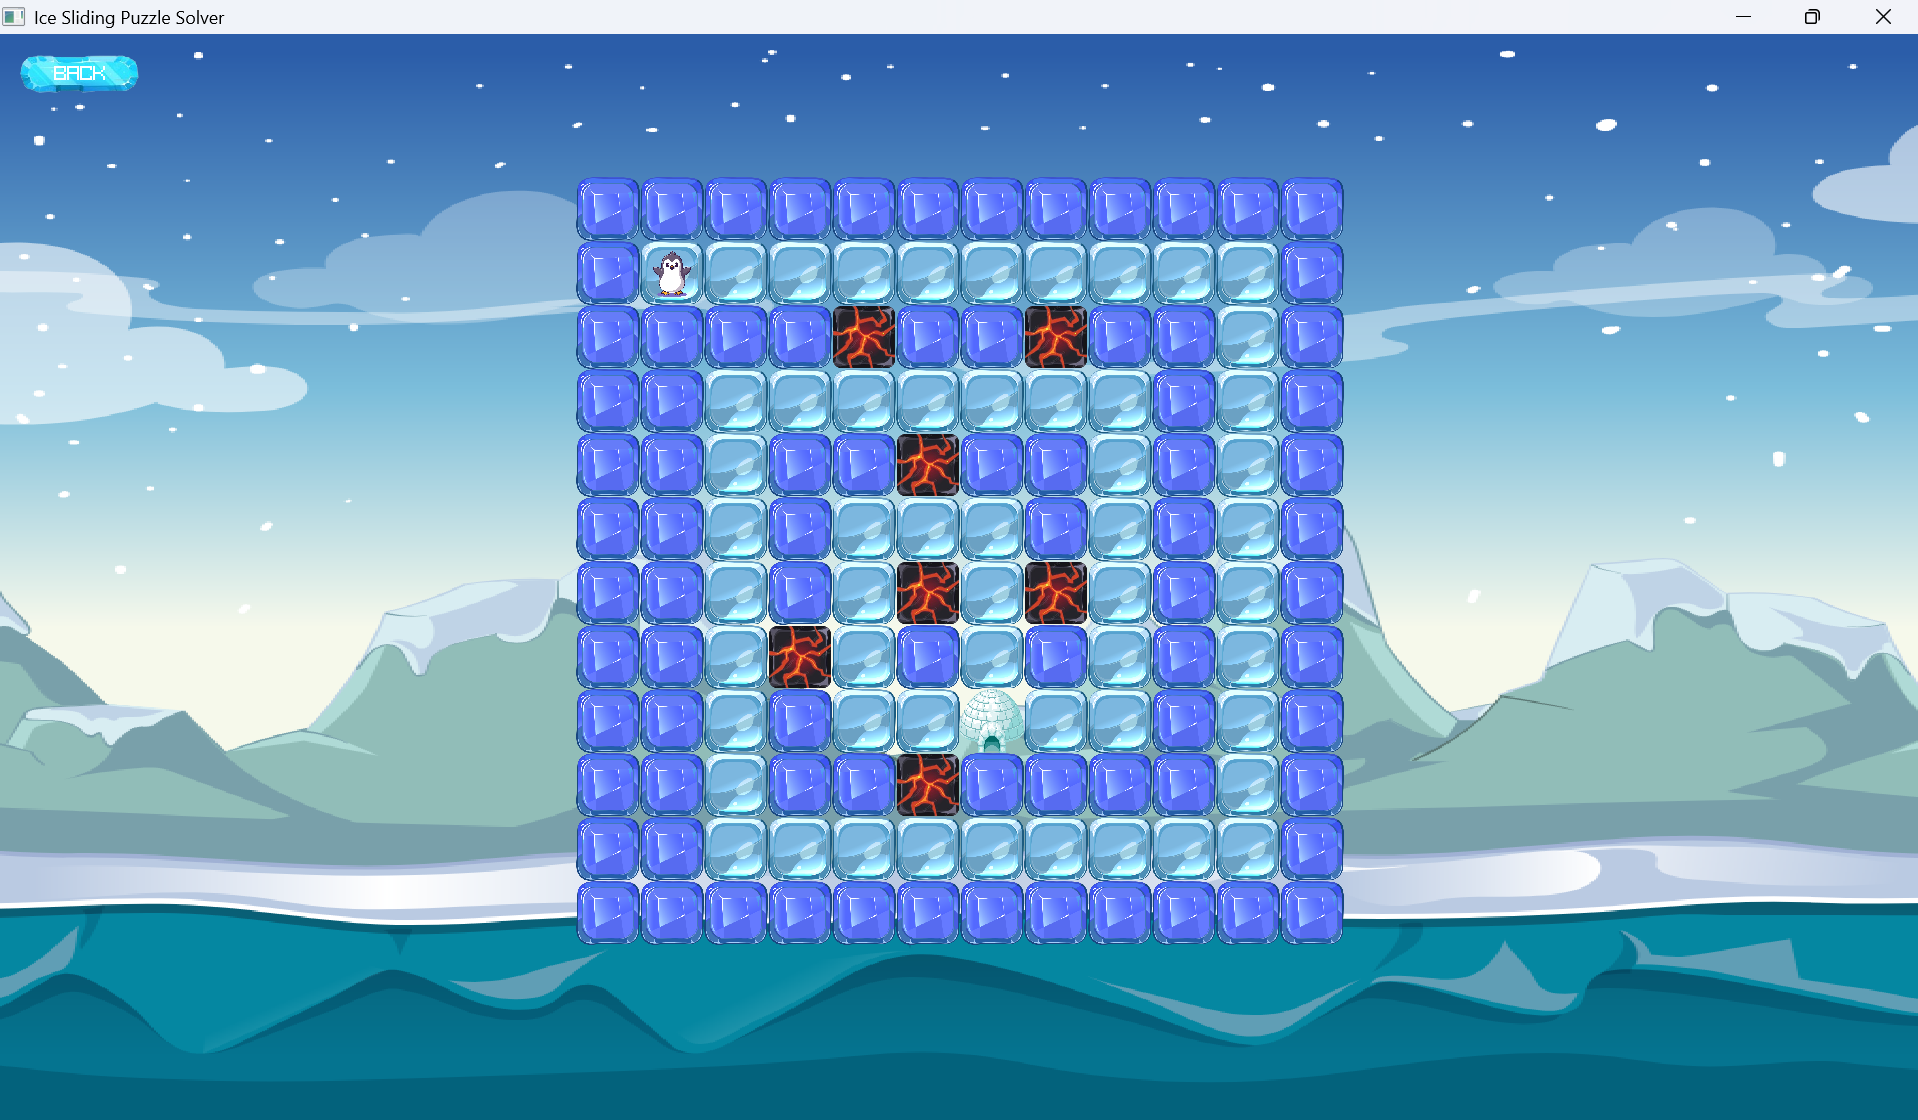
\includegraphics[width=0.65\textwidth]{public/map25.png}
	\caption{Visualisasi map pada Test Case 25}
\end{figure}

\begin{figure}[H]
	\centering
	\begin{minipage}{0.48\textwidth}
		\centering
		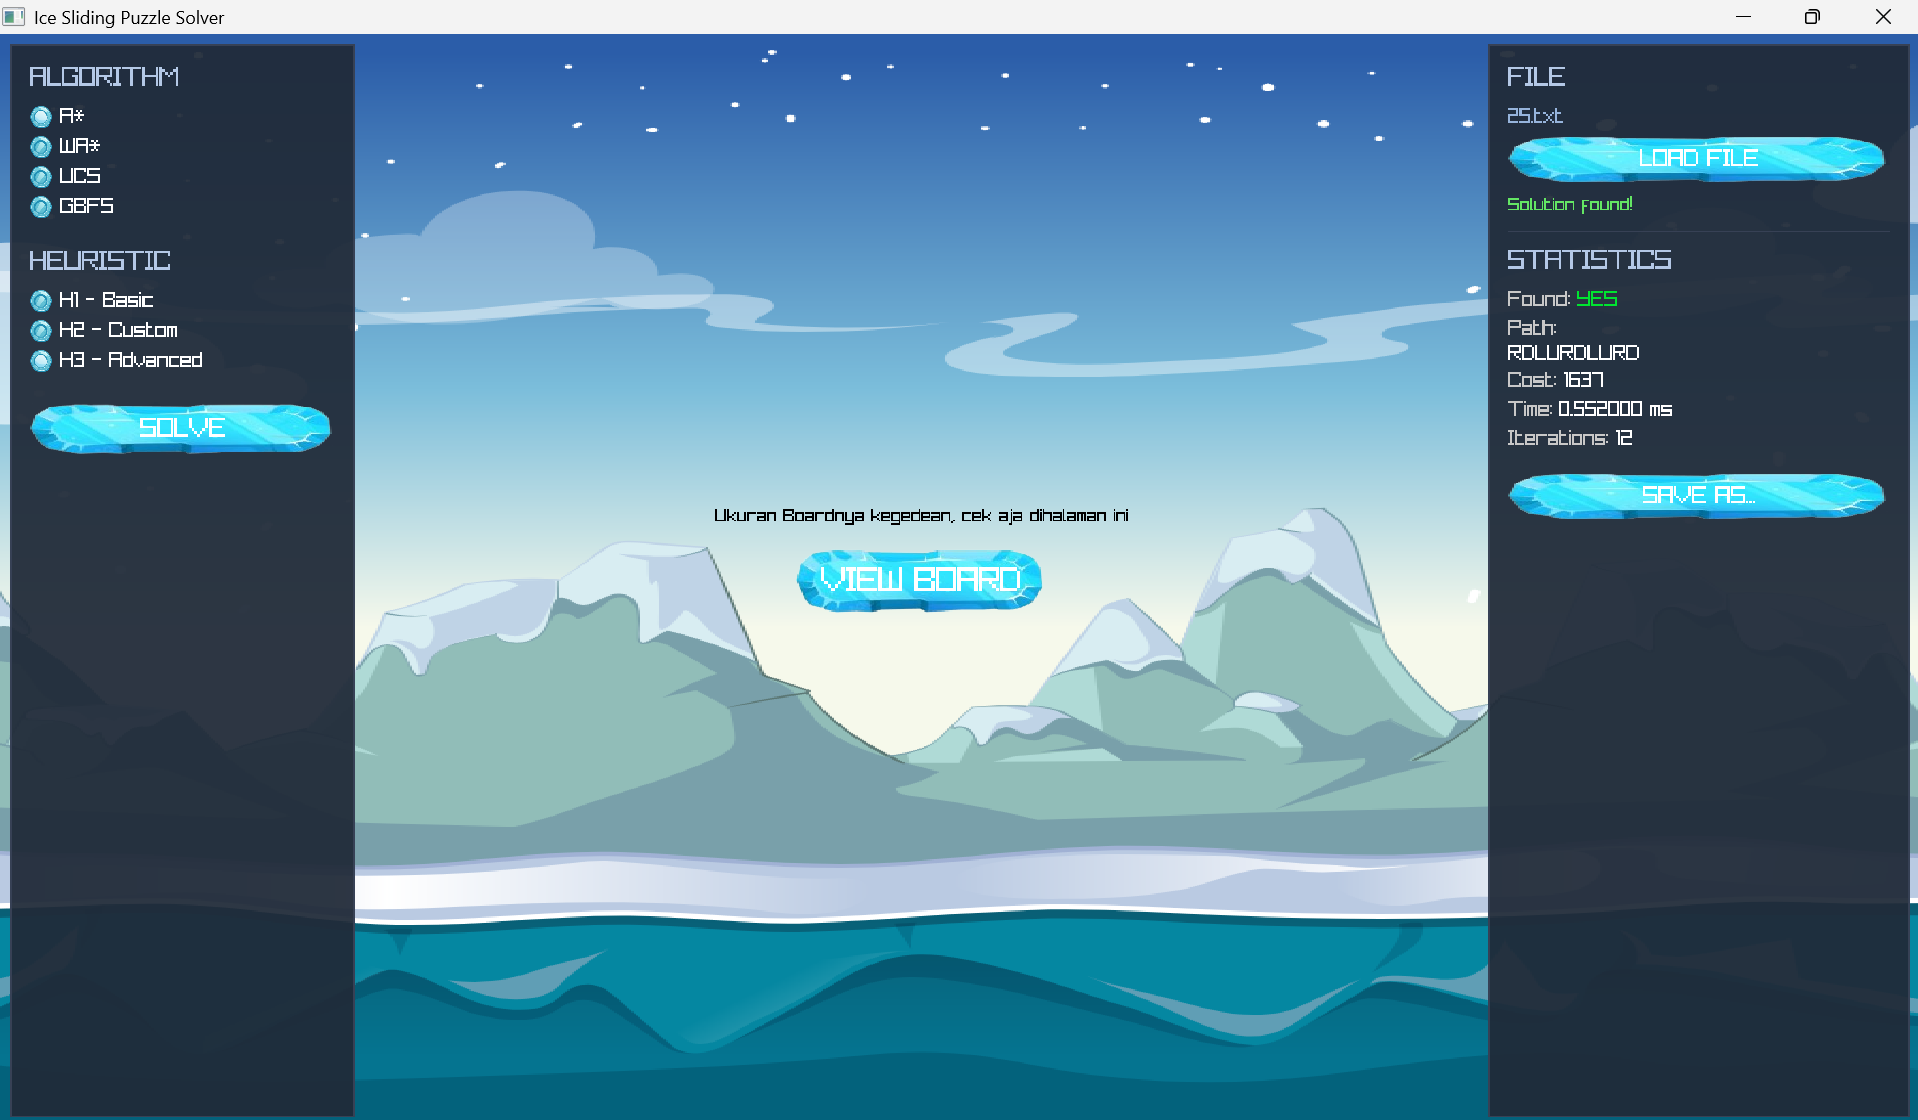
\includegraphics[width=\textwidth]{public/test25-A-h3.png}
		\caption{Output Test 25 menggunakan A* + H3}
	\end{minipage}
	\hfill
	\begin{minipage}{0.48\textwidth}
		\centering
		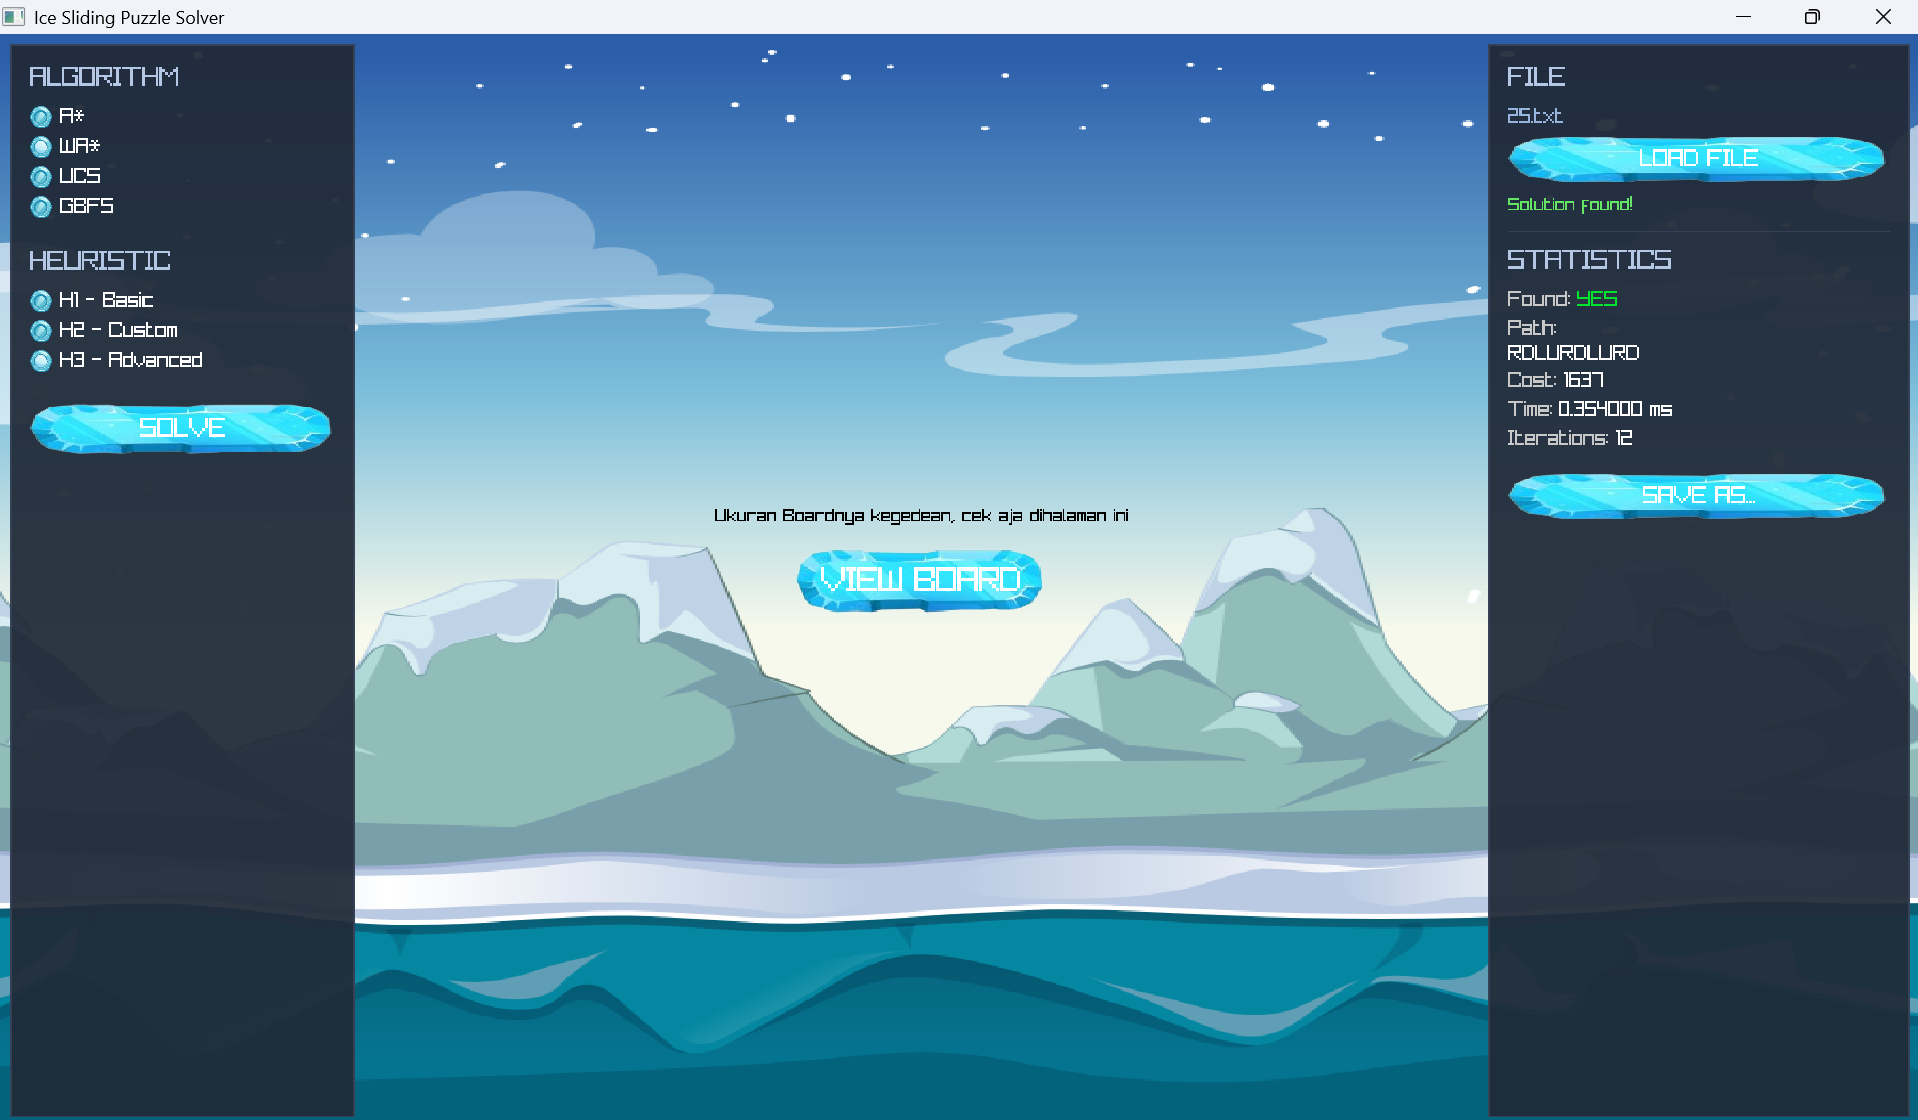
\includegraphics[width=\textwidth]{public/test25-WA-h3.png}
		\caption{Output Test 25 menggunakan Weighted A* + H3}
	\end{minipage}
\end{figure}

\begin{table}[H]
	\centering
	\caption{Hasil percobaan pada Test Case 25}
	\small
	\begin{tabular}{|p{4cm}|p{2.5cm}|p{2.5cm}|p{2.5cm}|}
		\hline
		\rowcolor{gray!20}
		\textbf{Algoritma} & \textbf{Cost} & \textbf{Time (ms)} & \textbf{Iterations} \\
		\hline
		A* - Basic & 1637 & 0.219 & 12 \\
		\hline
		A* - Custom & 1637 & 0.730 & 12 \\
		\hline
		A* - Advanced & 1637 & 0.949 & 12 \\
		\hline
		WA* - Basic & 1637 & 0.202 & 12 \\
		\hline
		WA* - Custom & 1637 & 0.296 & 12 \\
		\hline
		WA* - Advanced & 1637 & 0.354 & 12 \\
		\hline
		UCS & 1637 & 0.159 & 11 \\
		\hline
		GBFS - Basic & 1637 & 0.207 & 11 \\
		\hline
		GBFS - Custom & 1637 & 0.390 & 11 \\
		\hline
		GBFS - Advanced & 1637 & 0.388 & 11 \\
		\hline
	\end{tabular}
\end{table}

\begin{tcolorbox}[
	colback=green!5,
	colframe=green!50!black,
	title=\textbf{Ringkasan Test Case 25},
	arc=2mm,
	boxrule=0.8pt
]
Seluruh algoritma menghasilkan cost solusi yang sama, yaitu 1637. 
Meskipun map memiliki banyak lava dan obstacle, semua algoritma tetap dapat menemukan solusi valid. 
Perbedaan utama terlihat pada waktu eksekusi dan jumlah iterasi, bukan pada total cost solusi.
\end{tcolorbox}


\section{Ringkasan Hasil Tangkapan Layar}

Berdasarkan lima test case yang ditampilkan, program berhasil membaca input, menjalankan algoritma yang dipilih, dan menghasilkan output berupa solusi, cost, waktu eksekusi, serta jumlah iterasi. 
Setiap test case juga dilengkapi dengan visualisasi map dan dua tangkapan layar output sebagai bukti bahwa program dapat dijalankan pada beberapa konfigurasi papan yang berbeda.

\begin{table}[H]
	\centering
	\caption{Ringkasan pasangan tangkapan layar yang digunakan}
	\begin{tabular}{|p{2.2cm}|p{4.3cm}|p{4.3cm}|p{3cm}|}
		\hline
		\rowcolor{blue!15}
		\textbf{Test Case} & \textbf{Screenshot 1} & \textbf{Screenshot 2} & \textbf{Status} \\
		\hline
		Test 8 & GBFS + H3 & Weighted A* + H2 & Berhasil \\
		\hline
		Test 17 & GBFS + H1 & Weighted A* + H1 & Berhasil \\
		\hline
		Test 20 & A* + H1 & UCS & Berhasil \\
		\hline
		Test 24 & A* + H2 & GBFS + H2 & Berhasil \\
		\hline
		Test 25 & A* + H3 & Weighted A* + H3 & Berhasil \\
		\hline
	\end{tabular}
\end{table}